\documentclass{article}
\usepackage{makeidx}
\usepackage{hyperref}
\usepackage{amsmath}
\usepackage{amssymb}
\usepackage{xcolor}
\usepackage{graphicx}
\usepackage[top=1in, bottom=1in, left=1in, right=1in]{geometry}

\title{Machine Learning Notes}
\author{chtunsw@gmail.com}
\date{}

\makeatletter
\renewcommand\paragraph{\@startsection{paragraph}{4}{\z@}%
                                     {-3.25ex\@plus -1ex \@minus -.2ex}%
                                     {1.5ex \@plus .2ex}%
                                     {\normalfont\normalsize\bfseries}}
\makeatletter

\hypersetup{
    colorlinks=true,
    linkcolor=blue,
    urlcolor=cyan,
}

\setcounter{tocdepth}{4}
\setcounter{secnumdepth}{4}

\makeindex



\begin{document}

\maketitle

\clearpage

\tableofcontents{}

\clearpage

\section{Machine Learning Introduction}

A computer program is said to learn
from experience E with respect to some task T
and some performance measure P, if its
performance on T, as measured by P, improves
with experience E. 

\subsection{Supervised Learning}

Supervised learning algorithms build a mathematical model 
of a set of data that contains both the inputs and the desired 
outputs.

\bigskip

\noindent In supervised learning, each example is a 
pair consisting of an input object (typically a vector) 
and a desired output value (also called the supervisory signal).

\subsubsection{Regression}

Regression analysis is a set of statistical processes 
for estimating the relationships between a dependent 
variable (often called the `outcome variable') and one 
or more independent variables (often called `predictors', 
`covariates', or `features').

\bigskip

\noindent \textbf{Training(Learning) Process:}

\noindent \textit{observed data(training set)} $\rightarrow$ \textit{learning algorithm} $\rightarrow$ \textit{h(hypothesis)}

\bigskip

\noindent \textbf{Predicting Process:}

\noindent \textit{independent variable} $\rightarrow$ \textit{h(hypothesis)} $\rightarrow$ \textit{dependent variable}

\subsubsection{Classification}

Classification is the problem of identifying to which 
of a set of categories (sub-populations) a new observation 
belongs, on the basis of a training set of data containing 
observations (or instances) whose category membership is known.

\subsection{Unsupervised Learning}

Unsupervised learning algorithms take a set of data that 
contains only inputs, and find structure in the data, like 
grouping or clustering of data points.

\bigskip

\noindent Draw inferences from data sets consisting of input 
data without labeled responses.

\subsection{Reinforcement learning}
       
Reinforcement learning is an area of machine learning concerned 
with how software agents ought to take actions in an environment 
so as to maximize some notion of cumulative reward.

\section{Regression}

\subsection{Linear Regression(from \href{https://en.wikipedia.org/wiki/Linear_regression\#:~:text=In\%20statistics\%2C\%20linear\%20regression\%20is,is\%20called\%20simple\%20linear\%20regression.}{Wikipedia})}

Given a data set \(\{y_i, x_{i1}, ..., x_{ip}\}_{i=1}^n\) of n statistical units, a linear regression model assumes that the relationship between the dependent variable y and the p-vector of regressors x is linear.

\[y_i = \beta_0 + \beta_{1}x_{i1} + \dots + \beta_{p}x_{ip} + \epsilon_i, \: i = 1, \dots, n\]
\[y = X\beta + \epsilon\]

\noindent where

\bigskip

\(
y = 
\begin{bmatrix}
y_1\\
y_2\\
\vdots\\
y_n
\end{bmatrix}
,
X = 
\begin{bmatrix}
x_1^T\\
x_2^T\\
\vdots\\
x_n^T
\end{bmatrix} = 
\begin{bmatrix}
1 & x_{11} & \dots & x_{1p}\\
1 & x_{21} & \dots & x_{2p}\\
\vdots & \vdots & \ddots & \vdots\\
1 & x_{n1} & \dots & x_{np}
\end{bmatrix}
,
\beta = 
\begin{bmatrix}
\beta_0\\
\beta_1\\
\vdots\\
\beta_p
\end{bmatrix}
,
\epsilon = 
\begin{bmatrix}
\epsilon_1\\
\epsilon_2\\
\vdots\\
\epsilon_n
\end{bmatrix}
\)

\bigskip

\noindent \(y\) is a vector of observed values \(y_{i}\ (i=1,\ldots ,n)\) of the variable called the regressand, endogenous variable, response variable, measured variable, criterion variable, or dependent variable.

\bigskip

\noindent \(X\) may be seen as a matrix of row-vectors \(x_{i}\) or of n-dimensional column-vectors \(X_{j}\), which are known as regressors, exogenous variables, explanatory variables, covariates, input variables, predictor variables, or independent variables. Usually a constant is included as one of the regressors. In particular, \(x_{i0} = 1\) for \(i = 1, \dots, n\). The corresponding element of \(\beta\) is called the intercept. 

\bigskip

\noindent \(\beta\) is a \((p + 1)\)-dimensional parameter vector, where \(\beta_{0}\) is the intercept term (if one is included in the model—otherwise \(\beta\) is p-dimensional). Its elements are known as effects or regression coefficients (although the latter term is sometimes reserved for the estimated effects).

\bigskip

\noindent \(\epsilon\) is a vector of values \(\epsilon_{i}\). This part of the model is called the error term, disturbance term, or sometimes noise (in contrast with the ``signal" provided by the rest of the model).

\bigskip

\noindent \textbf{Matrix Concepts}

\bigskip

\noindent \textbf{identity matrix} \(I\)(or \(I_{n \times n}\)):

\[A \cdot I = I \cdot A = A\]

\[
I = 
\begin{bmatrix}
1 & 0 & \dots & 0 & 0\\
0 & 1 & \dots & 0 & 0\\
\vdots & \vdots & \ddots & \vdots & \vdots\\
0 & 0 & \dots & 1 & 0\\
0 & 0 & \dots & 0 & 1
\end{bmatrix}
\]

\noindent \textbf{inverse matrix} \(A^{-1}\): If \(A\) is an \(m \times m\) matrix, and if it has an inverse.
\[A \cdot A^{-1} = A^{-1} \cdot A = I\]

\noindent \textbf{transpose matrix} \(A^{T}\): Let \(A\) be an \(m \times n\) matrix. Then \(A^T\) is an \(n \times m\) matrix.
\[A^T_{ij} = A_{ji}\]

\subsubsection{Linear Regression Learning (from \href{https://www.coursera.org/learn/machine-learning}{Machine Learning course})}

\noindent For convenience reasons, define \(x_0 = 1\)
\[
x = 
\begin{bmatrix}
x_0\\
x_1\\
\vdots\\
x_n
\end{bmatrix}
,
\theta = 
\begin{bmatrix}
\theta_0\\
\theta_1\\
\vdots\\
\theta_n
\end{bmatrix}
\]

\noindent \textbf{hypothesis}:
\[y = h_{\theta}(x) = \theta^T x = \theta_0 + \theta_1 x_1 + \theta_2 x_2 + \dots + \theta_n x_n\]

\noindent \textbf{training data}:
\[(x^{(i)}, y^{(i)})\:for\:i = 1, \dots, m\]

\noindent \textbf{cost function}:

\noindent convex: second derivative (hessian matrix) is non-negative definite.

\noindent goal: \(\underset{\theta}{\text{minimize}} \: J(\theta)\)
\[J(\theta) = \frac{1}{2m} \sum_{i = 1}^m (h_{\theta}(x^{(i)}) - y^{(i)})^2\]

\noindent \textbf{gradient descent}:

\noindent repeat until convergence \{
\[\theta_j =: \theta_j - \alpha \frac{\partial}{\partial \theta_j} J(\theta) = \theta_j - \alpha \frac{1}{m} \sum_{i = 1}^m (h_{\theta}(x^{(i)}) - y^{(i)}) x^{(i)}_j\]
\centerline{simultaneously update \(\theta_j\) for \(j = 0, \dots, n\)}
\}

\bigskip

\noindent \textbf{vectorized implementation}:

\noindent repeat until convergence \{
\[\theta =: \theta - \alpha \frac{1}{m} \sum_{i = 1}^m (h_{\theta}(x^{(i)}) - y^{(i)}) x^{(i)}\]
\}

\bigskip

\noindent \textbf{batch size}:

\noindent The number of training samples to use in a training action.

\bigskip

\noindent \textbf{epoch}:

\noindent The number of times of training which uses all the training samples.

\bigskip

\noindent \textbf{Feature scaling}:

\noindent The range of all features should be normalized so that each feature contributes approximately proportionately to the result. Also it helps gradient descent converge much faster.

\bigskip

\noindent \textbf{mean normalization}: (don't apply to \(x_0\))

\[x_i = \frac{x_i - mean(x_i)}{max(x_i) - min(x_i)}\]

\bigskip

\noindent \textbf{standardization}: (don't apply to \(x_0\))

\noindent Feature standardization makes the values of each feature in the data have zero-mean (when subtracting the mean in the numerator) and unit-variance.

\[\mu: \text{mean, } \sigma^2: \text{variance, } \sigma: \text{standard deviation}\]

\[\mu_i ={\frac {1}{m}}\sum _{j=1}^{m}x^{(j)}_{i}\]

\[\sigma^2_i = \frac{1}{m} \sum_{j = 1}^m (x^{(j)}_i - \mu_i)^2\]

\[x_i = \frac{x_i - \mu_i}{\sigma_i}\]

\noindent \textbf{learning rate} \(\alpha\):

\noindent If \(\alpha\) is too small: slow convergence.

\noindent If \(\alpha\) is too large: may not decrease on every iteration and thus may not converge.

\noindent try a range of learning rate to find a good one:

\[\alpha = \dots, 0.001, \dots, 0.01, \dots, 0.1, \dots\]

\noindent \textbf{Feature choosing}:

\noindent Choose the right features to fit the data set.

\noindent housing price example, choose from:

\[h_{\theta}(x) = \theta_0 + \theta_1 \times frontage + \theta_2 \times depth\]
\[h_{\theta}(x) = \theta_0 + \theta_1 \times area\]

\noindent \textbf{polynomial regression}:

\noindent Use the polynomial model with the machinery of multivariant linear regression.

\noindent housing price example, choose from:

\[h_{\theta}(x) = \theta_0 + \theta_1 \times area + \theta_2 \times area^2\]
\[h_{\theta}(x) = \theta_0 + \theta_1 \times area + \theta_2 \times \sqrt{area}\]

\subsubsection{Normal Equation}

\noindent Let:

\[
X = 
\begin{bmatrix}
(x^{(1)})^T\\
(x^{(2)})^T\\
\vdots\\
(x^{(m)})^T
\end{bmatrix}
,
y = 
\begin{bmatrix}
y^{(1)}\\
y^{(2)}\\
\vdots\\
y^{(m)}
\end{bmatrix}
\]

\noindent Calculate best \(\theta\): \textcolor{orange}{ * maths derivation needed}

\[
\theta = (X^TX)^{-1}X^Ty
\]

\noindent If \(X^TX\) is noninvertible, the common causes might be having:

\noindent 1. Redundant features, where two features are very closely related (i.e. they are linearly dependent)

\noindent 2. Too many features (e.g. \(m < n\)). In this case, delete some features or use "regularization".

\bigskip

\noindent \textbf{Gradient Descent} vs \textbf{Normal Equation}:

\begin{center}
\begin{tabular}{ | c | c | } 
\hline
\textbf{Gradient Descent} & \textbf{Normal Equation} \\ 
\hline
Need to choose \(\alpha\) & No need to choose \(\alpha\) \\ 
\hline
Needs many iterations & No need to iterate \\ 
\hline
\(O(kn^2)\) & \(O(n^3)\). Need to calculate \((X^TX)^{-1}\) \\ 
\hline
Works well when n is large & Slow if n is very large \\ 
\hline
\end{tabular}
\end{center}

\noindent \textbf{Vectorized Cost Function}:

\[J(\theta) = \frac{1}{2m} (X\theta - y)^T(X\theta - y)\]

\subsection{Logistic Regression}

\noindent \textbf{sigmoid function:} (Logistic Function)

\noindent Maps any real number from \((-\infty, +\infty)\) to the \((0, 1)\) interval.
\[g(z) = \frac{1}{1 + e^{-z}}\]

\noindent \textbf{hypothesis:}
\[
h_{\theta}(x) 
= g(\theta^T x)
= \frac{1}{1 + e^{-\theta^T x}}
\]

\noindent \(h_{\theta}(x)\) will give us the probability that our output is 1. Our probability that our prediction is 0 is just the complement of our probability that it is 1.

\[
h_{\theta} (x) 
= P(y = 1 \mid x ; \theta)
= 1 - P(y = 0 \mid x ; \theta)
\]
\[P(y = 1 \mid x ; \theta) + P(y = 0 \mid x ; \theta) = 1\]

\noindent \textbf{decision boundary:}

\noindent In order to get our discrete 0 or 1 classification, we can translate the output of the hypothesis function as follows:

\[h_{\theta} (x) \geq 0.5 \rightarrow y = 1\]
\[h_{\theta} (x) < 0.5 \rightarrow y = 0\]

\noindent Decision is made when:

\[g(\theta^T x) \geq 0.5, \text{ when } \theta^T x \geq 0\]
\[g(\theta^T x) < 0.5, \text{ when } \theta^T x < 0\]

\noindent Now we get:

\[\theta^T x \geq 0 \rightarrow y = 1\]
\[\theta^T x < 0 \rightarrow y = 0\]

\noindent The decision boundary is the line that separates the area where \(y = 0\) and where \(y = 1\):
\[\theta^T x = 0\]

\noindent \textbf{cost function:}

\noindent If we use the the same cost function that we use for linear regression for logistic regression, the cost function will have many local optima. It will not be a convex function. Instead, we construct logistic regression cost function as follows:

\[J(\theta) = \frac{1}{m} \sum_{i = 1}^m Cost(h_{\theta}(x^{(i)}), y^{(i)})\]
\[Cost(h_{\theta}(x), y) = -log(h_{\theta}(x)), \text{ if } y = 1\]
\[Cost(h_{\theta}(x), y) = -log(1 - h_{\theta}(x)), \text{ if } y = 0\]

\noindent We can find it guarantees that \(J(\theta)\) is convex for logistic regression:
\[
Cost(h_{\theta}(x), y) = 0 \text{ if }
h_{\theta}(x) = y, \text{ at } h_{\theta}(x) = y = 0 \text{ and } 
h_{\theta}(x) = y = 1
\]
\[
Cost(h_{\theta}(x), y) \rightarrow +\infty
\text{ if } y = 0 \text{ and }
h_{\theta}(x) \rightarrow 1
\]
\[
Cost(h_{\theta}(x), y) \rightarrow +\infty
\text{ if } y = 1 \text{ and }
h_{\theta}(x) \rightarrow 0
\]

\noindent We can compress our cost function's two conditional cases into one case:
\[Cost(h_{\theta} (x), y) 
= - y log(h_{\theta} (x)) - (1 - y) log(1 - h_{\theta} (x))\]

\noindent \textbf{simplified cost function:}
\[J(\theta) = - \frac{1}{m} \sum_{i = 1}^{m} [y^{(i)} log(h_{\theta} (x^{(i)})) + (1 - y^{(i)}) log(1 - h_{\theta} (x^{(i)}))]\]

\noindent \textbf{vectorized cost function:}
\[h = g(X\theta)\]
\[J(\theta) = \frac{1}{m} (- y^T log(h) - (1 - y)^T log(1 - h))\]

\noindent \textbf{gradient descent:}

\noindent repeat until convergence \{
\[\theta_j =: \theta_j - \alpha \frac{\partial}{\partial \theta_j} J(\theta) = \theta_j - \alpha \frac{1}{m} \sum_{i = 1}^m (h_{\theta}(x^{(i)}) - y^{(i)}) x^{(i)}_j\]
\centerline{simultaneously update \(\theta_j\) for \(j = 0, \dots, n\)}
\}

\bigskip

\noindent \textbf{vectorized implementation}:

\noindent repeat until convergence \{
\[\theta =: \theta - \alpha \frac{1}{m} X^T (g(X\theta) - y)\]
\}

\bigskip

\noindent \textbf{advanced optimization methods}:

\noindent With the same cost function, we can choose different optimization method to optimize \(\theta\):

\begin{itemize}
\item gradient descent
\item conjugate gradient
\item BFGS
\item L-BFGS
\item ...
\end{itemize}

\bigskip

\noindent \textbf{multiclass classification: (one vs all)}

\noindent Instead of \(y = \{0, 1\}\), we will expand our definition so that \(y = \{0, 1, ..., n\}\). Then we divide our problem into n+1 binary classification problems, by constructing n + 1 hypothesis functions; in each one, we choose one class and then lump all the others into a single second class, then predict the probability that \(y\) is a member of the chosen class.

\bigskip

\noindent To summarize: 

\noindent Train a logistic regression classifier \(h_{\theta}^{(i)}(x)\) for each class to predict the probability that \(y = i\). On a new input \(x\), to make a prediction, pick the class \(i\) that maximizes \(h_{\theta} ^{(i)}(x)\).

\[y \in \{0, 1 ... n\}\] 
\[h_{\theta}^{(0)}(x) = P(y = 0 \mid x ; \theta)\]
\[h_{\theta}^{(1)}(x) = P(y = 1 \mid x ; \theta)\]
\[\cdots\]
\[h_{\theta}^{(n)}(x) = P(y = n \mid x ; \theta)\] 
\[\text{prediction} = \max_i(h_{\theta}^{(i)}(x))\]

\subsection{Overfitting Problem}

\noindent \textbf{underfitting}:

\noindent High bias, which means hypothesis fits training data poorly, is usually caused by a function that is too simple or using too few features. 

\bigskip

\noindent \textbf{overfitting}:

\noindent High variance, which means hypothesis fits training data well, but does not generalize well to predict new data. It is usually caused by a complicated function with too many features.

\bigskip

\noindent \textbf{address overfitting}:

\begin{enumerate}
\item Reduce the number of features:
\begin{itemize}
\item Manually select which features to keep.
\item Use a model selection algorithm (studied later in the course).
\end{itemize}
\item Regularization:
\begin{itemize}
\item Keep all the features, but reduce the magnitude of parameters \(\theta_j\).
\item Regularization works well when we have a lot of slightly useful features.
\end{itemize}
\end{enumerate}

\subsubsection{Linear Regression Regularization}

\noindent \textbf{regularized cost function}:

\noindent We can reduce(penalize) the weight of the features in our function carry by increasing their cost. The \(\lambda\) is the regularization parameter. It determines how much the costs of our theta parameters are inflated. 

\[J(\theta) = \frac{1}{2m} \sum_{i = 1}^m (h_{\theta}(x^{(i)}) - y^{(i)})^2 + \frac{\lambda}{2m} \sum_{j = 1}^n \theta_j^2\]

\noindent Using the above cost function with the extra summation, we can smooth the output of our hypothesis function to reduce overfitting. If \(\lambda\) is too small, it would be hard to see a difference. If \(\lambda\) is too large, it may smooth out the function too much and cause underfitting.

\bigskip

\noindent \textbf{regularized gradient descent}:

\noindent repeat until convergence \{
\[\theta_0 =: \theta_0 - \alpha \frac{1}{m} \sum_{i = 1}^m (h_{\theta}(x^{(i)}) - y^{(i)}) x^{(i)}_0\]
\begin{equation*}
\begin{split}
\theta_j & =: \theta_j - \alpha ((\frac{1}{m} \sum_{i = 1}^m (h_{\theta}(x^{(i)}) - y^{(i)}) x^{(i)}_j) + \frac{\lambda}{m} \theta_j) \\
 & = \theta_j (1 - \alpha \frac{\lambda}{m}) - \alpha \frac{1}{m} \sum_{i = 1}^m (h_{\theta}(x^{(i)}) - y^{(i)}) x^{(i)}_j
\end{split}
\end{equation*}

\centerline{simultaneously update \(\theta_0\) and \(\theta_j\) for \(j = 1, \dots, n\)}
\}

\bigskip

\noindent The first term in the above equation, \(1 - \alpha \frac{\lambda}{m}\) will always be less than 1. Intuitively you can see it as reducing the value of \(\theta_j\) by some amount on every update.

\bigskip

\noindent \textbf{regularized normal equation}: \textcolor{orange}{ * maths derivation needed}

\[
\theta = (X^TX + \lambda L)^{-1}X^Ty
\]

\[
L = 
\begin{bmatrix}
0 & 0 & \dots & 0 & 0\\
0 & 1 & \dots & 0 & 0\\
\vdots & \vdots & \ddots & \vdots & \vdots\\
0 & 0 & \dots & 1 & 0\\
0 & 0 & \dots & 0 & 1
\end{bmatrix}
\]

\bigskip

\noindent L has a dimension of \((n + 1) \times (n + 1)\). Intuitively, this is the identity matrix (though we are not including \(x_0\) ), multiplied with a single real number \(\lambda\).

\bigskip

\noindent Recall that if \(m < n\), then \(X^TX\) is non-invertible. However, when we add the term \(\lambda L\) (\(\lambda > 0\)), the term \(X^TX + \lambda L\) becomes invertible.

\subsubsection{Logistic Regression Regularization}

\noindent \textbf{regularized cost function}:

\[J(\theta) = - \frac{1}{m} \sum_{i = 1}^{m} [y^{(i)} log(h_{\theta} (x^{(i)})) + (1 - y^{(i)}) log(1 - h_{\theta} (x^{(i)}))] + \frac{\lambda}{2m} \sum_{j = 1}^n \theta_j^2\]

\noindent \textbf{regularized gradient descent}:

\noindent repeat until convergence \{
\[\theta_0 =: \theta_0 - \alpha \frac{1}{m} \sum_{i = 1}^m (h_{\theta}(x^{(i)}) - y^{(i)}) x^{(i)}_0\]
\begin{equation*}
\begin{split}
\theta_j & =: \theta_j - \alpha ((\frac{1}{m} \sum_{i = 1}^m (h_{\theta}(x^{(i)}) - y^{(i)}) x^{(i)}_j) + \frac{\lambda}{m} \theta_j) \\
 & = \theta_j (1 - \alpha \frac{\lambda}{m}) - \alpha \frac{1}{m} \sum_{i = 1}^m (h_{\theta}(x^{(i)}) - y^{(i)}) x^{(i)}_j
\end{split}
\end{equation*}

\centerline{simultaneously update \(\theta_0\) and \(\theta_j\) for \(j = 1, \dots, n\)}
\}

\section{Neural Network}

\subsection{Basic Structure}

\begin{center}
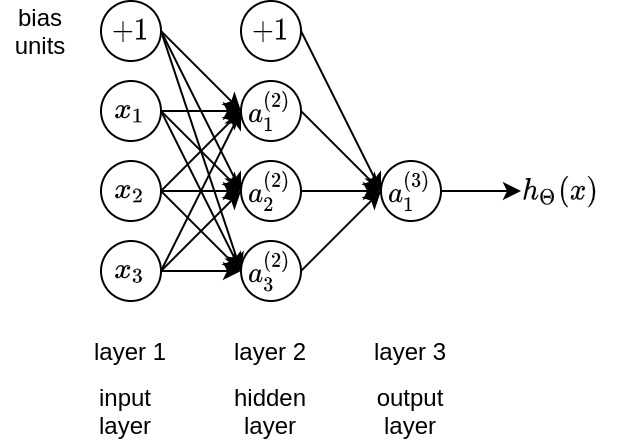
\includegraphics[scale=0.4]{./images/neural_network.jpg}
\end{center}
\[a_i^{(j)} = \text{"activation" of unit i in layer j}\]
\[\Theta^{(j)} = \text{matrix of weights (edges) from layer j to j + 1}\]

\bigskip

\[a_1^{(2)} = g(\Theta_{10}^{(1)} x_0 + \Theta_{11}^{(1)} x_1 + \Theta_{12}^{(1)} x_2 + \Theta_{13}^{(1)} x_3)\]
\[a_2^{(2)} = g(\Theta_{20}^{(1)} x_0 + \Theta_{21}^{(1)} x_1 + \Theta_{22}^{(1)} x_2 + \Theta_{23}^{(1)} x_3)\]
\[a_3^{(2)} = g(\Theta_{30}^{(1)} x_0 + \Theta_{31}^{(1)} x_1 + \Theta_{32}^{(1)} x_2 + \Theta_{33}^{(1)} x_3)\]
\[h_{\Theta}(x) = a_1^{(3)} = g(\Theta_{10}^{(2)} a_0^{(2)} + \Theta_{11}^{(2)} a_1^{(2)} + \Theta_{12}^{(2)} a_2^{(2)} + \Theta_{13}^{(2)} a_3^{(2)})\]

\bigskip

\noindent If network has \(s_j\) units in layer \(j\), \(s_{j + 1}\) units in layer \(j + 1\), then \(\Theta^{(j)}\) will be of dimension \(s_{j + 1} \times (s_j + 1)\).

\subsection{Simple Applications}

\begin{center}
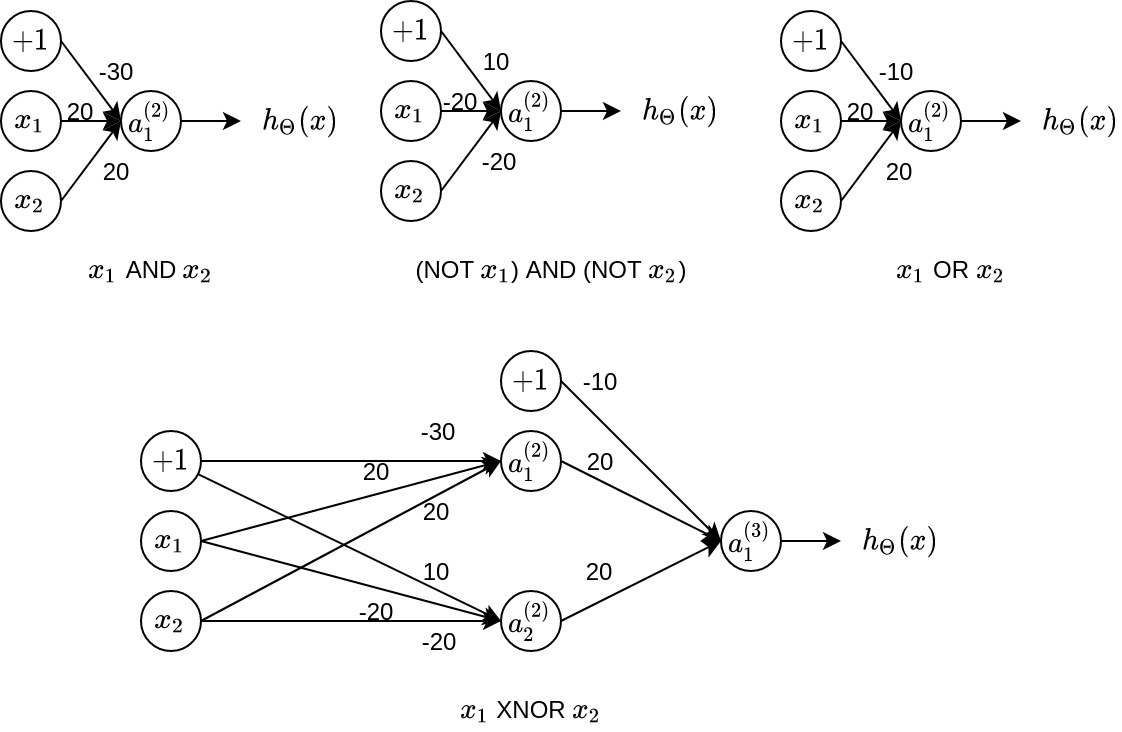
\includegraphics[scale=0.3]{./images/neural_network_simple_applications.jpg}
\end{center}

\subsection{Generalized Model (one vs all)}

\begin{center}
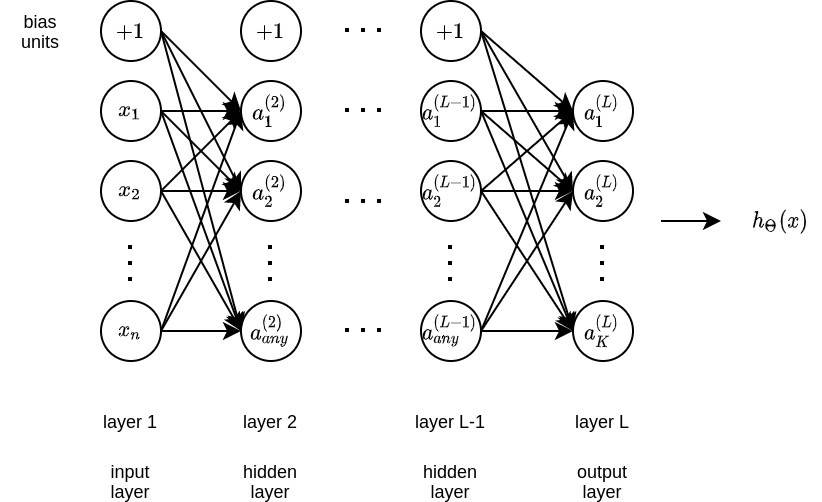
\includegraphics[scale=0.4]{./images/neural_network_generalized.jpg}
\end{center}

\noindent For a neural network that has:

\[L = \text{total number of layers in the network}\]
\[s_l = \text{number of units (not counting bias unit) in layer } l\]
\[K = \text{number of output units/classes}\]

\noindent assume \(a^{(1)} = x, a^{(L)} = h_\Theta(x)\), let:

\[z^{(l)} = \Theta^{(l - 1)} a^{(l - 1)}\]
\[a^{(l)} = g(z^{(l)})\]
\[h_\Theta(x) = a^{(L)} = g(z^{(L)})\]

\noindent Notice that bias units (\(a_0^{(l)} = 1\)) are considered as input only when calculating the next layer. They are not included in the output generated by previous layer.

\bigskip

\noindent \textbf{regularized cost function:}
\[J(\Theta) = - \frac{1}{m} \sum_{i = 1}^{m} \sum_{k = 1}^{K} [y^{(i)}_k log(h_{\Theta} (x^{(i)})_k) + (1 - y^{(i)}_k) log(1 - h_{\Theta}(x^{(i)})_k)] + \frac{\lambda}{2m} \sum_{l = 1}^{L - 1} \sum_{i = 1}^{s_l} \sum_{j = 1}^{s_{l + 1}} (\Theta_{j, i}^{(l)})^{2}\]

\subsection{Backpropagation Preliminary}
\noindent \textbf{matrix calculus:} see \href{https://en.wikipedia.org/wiki/Matrix_calculus}{Wikipedia}

\noindent \textbf{chaine rule:}

\noindent Suppose the variable \(J\) depends on the variables \(\theta_1, \dots, \theta_p\) via the intermediate variable \(z_1, \dots, z_k\).

\[z_j = z_j(\theta_1, \dots, \theta_p), \forall j \in \{1, \dots, k\} \]
\[J = J(z_1, \dots, z_k)\]

\noindent Expand \(J\), we can find:

\[\frac{\partial J}{\partial \theta_i} = \sum_{j = 1}^{k} \frac{\partial J}{\partial z_j} \frac{\partial z_j}{\partial \theta_i}, \forall i \in \{1, \dots, p\}\]

\noindent \textbf{chain rule derivation for matrix:}

\noindent Suppose \(J\) is a real-valued output variable, \(z \in \mathbb{R}^m\) is the intermediate variable and \(\Theta \in \mathbb{R}^{m \times d}\), \(a \in \mathbb{R}^d\) are the input variables. Suppose they satisfy:

\[z = \Theta a\]
\[J = J(z)\]

\noindent Then we can get:

\[
\frac{\partial J}{\partial a} = 
\begin{bmatrix}
\frac{\partial J}{\partial a_1}\\
\vdots\\
\frac{\partial J}{\partial a_d}
\end{bmatrix}
= 
\begin{bmatrix}
\sum_{j = 1}^m \frac{\partial J}{\partial z_j} \frac{z_j}{a_1}\\
\vdots\\
\sum_{j = 1}^m \frac{\partial J}{\partial z_j} \frac{z_j}{a_d}
\end{bmatrix}
=
\begin{bmatrix}
\frac{\partial z_1}{\partial a_1} & \dots & \frac{\partial z_m}{\partial a_1}\\
\vdots & \ddots & \vdots\\
\frac{\partial z_1}{\partial a_d} & \dots & \frac{\partial z_m}{\partial a_d}
\end{bmatrix}
\begin{bmatrix}
\frac{\partial J}{\partial z_1}\\
\vdots\\
\frac{\partial J}{\partial z_m}
\end{bmatrix}
= \frac{\partial z}{\partial a} \frac{\partial J}{\partial z}
= \Theta^T \frac{\partial J}{\partial z}
\]

\[
\frac{\partial J}{\partial \Theta_{ij}} = \sum_{k = 1}^m \frac{\partial J}{\partial z_k} \frac{\partial z_k}{\partial \Theta_{ij}} = \frac{\partial J}{\partial z_i} \frac{\partial z_i}{\partial \Theta_{ij}} = \frac{\partial J}{\partial z_i} a_j
\]

\[
\frac{\partial J}{\partial \Theta} = 
\begin{bmatrix}
\frac{\partial J}{\partial z_1}\\
\vdots\\
\frac{\partial J}{\partial z_m}
\end{bmatrix}
\begin{bmatrix}
a_1 & \dots & a_d
\end{bmatrix}
= \frac{\partial J}{\partial z} a^T
\]

\noindent \textbf{element-wise chain rule:}

\noindent Assume \(z, a \in \mathbb{R}^d\):

\[a = \sigma(z) \text{, where \(\sigma\) is an element-wise activation}\]
\[J = J(a)\]

\noindent Then we have:

\[\frac{\partial J}{\partial z} = \frac{\partial J}{\partial a} \odot \sigma'(z)\]

\noindent Where \(\sigma'\) is the element-wise derivative of the activation function \(\sigma\).

\subsection{Backpropagation}

\noindent To train the model, we need to update \(\Theta\) for each epoch: (gradient decent)

\[\Theta := \Theta - \alpha  \frac{\partial}{\partial \Theta} J(\Theta)\]

\noindent We can see \(\frac{\partial}{\partial \Theta} J(\Theta)\) is hard to get directly. There is an easier way to calculate it. For each training example \((x^{(q)}, y^{(q)}), q \in \{1, \dots, m\}\), define \textbf{loss function}:

\[J = -\sum_{k = 1}^{K} [y^{(q)}_k log(h_{\Theta} (x^{(q)})_k) + (1 - y^{(q)}_k) log(1 - h_{\Theta}(x^{(q)})_k)] \]

\noindent Apply chain rule we have:

\[\frac{\partial J}{\partial \Theta^{(l)}} = \frac{\partial J}{\partial z^{(l + 1)}} (a^{(l)})^T\]
\[\frac{\partial J}{\partial a^{(l)}} = (\Theta^{(l)})^T \frac{\partial J}{\partial z^{(l + 1)}}\]
\begin{equation*}
\begin{split}
\frac{\partial J}{\partial z^{(l)}}
& = \frac{\partial J}{\partial a^{(l)}} \odot g'(z^{(l)}) \\
& = (\Theta^{(l)})^T \frac{\partial J}{\partial z^{(l + 1)}} \odot g'(z^{(l)}) \\
& = (\Theta^{(l)})^T \frac{\partial J}{\partial z^{(l + 1)}} \odot (a^{(l)} \odot (1 - a^{(l)}))
\end{split}
\end{equation*}

\noindent For \(p \in \{1, ..., K\}\):
\begin{equation*}
\begin{split}
\frac{\partial J}{\partial z_p^{(L)}} 
& = \frac{\partial}{\partial z_p^{(L)}} \sum_{k = 1}^{K} -[y^{(q)}_k log(h_{\Theta} (x^{(q)})_k) + (1 - y^{(q)}_k) log(1 - h_{\Theta}(x^{(q)})_k)] \\
& = \frac{\partial}{\partial z_p^{(L)}} \{-[y^{(q)}_p log(\frac{1}{1 + e^{-z_p^{(L)}}}) + (1 - y^{(q)}_p) log(1 - \frac{1}{1 + e^{-z_p^{(L)}}})]\} \\
& = - [y^{(q)}_p (1 + e^{-z_p^{(L)}}) \frac{0 - (-e^{-z_p^{(L)}})}{(1 + e^{-z_p^{(L)}})^2} + (1 - y^{(q)}_p) \frac{1 + e^{-z_p^{(L)}}}{e^{-z_p^{(L)}}} \frac{(-e^{-z_p^{(L)}})(1 + e^{-z_p^{(L)}}) - e^{-z_p^{(L)}}(-e^{-z_p^{(L)}})}{(1 + e^{-z_p^{(L)}})^2}] \\
& = - [y_p^{(q)} \frac{e^{-z_p^{(L)}}}{1 + e^{-z_p^{(L)}}} + (1 - y_p^{(q)}) \frac{-1}{1 + e^{-z_p^{(L)}}}] \\
& = - \frac{y_p^{(q)}e^{-z_p^{(L)}} + y_p^{(q)} - 1}{1 + e^{-z_p^{(L)}}} \\
& = \frac{1}{1 + e^{-z_p^{(L)}}} - y_p^{(q)} \\ 
& = a_p^{(L)} - y_p^{(q)}
\end{split}
\end{equation*}

\noindent Then we get:

\[\frac{\partial J}{\partial z^{(L)}} = 
\begin{bmatrix}
\frac{\partial J}{\partial z_1^{(L)}} \\
\vdots \\
\frac{\partial J}{\partial z_K^{(L)}}
\end{bmatrix}
= a^{(L)} - y^{(q)}
\]

\noindent For convenience, define \textbf{error term}: 
\[\delta^{(l)} = \frac{\partial J}{\partial z^{(l)}}\]

\noindent Then we get:

\[\frac{\partial J}{\partial \Theta^{(l)}} = \delta^{(l + 1)} (a^{(l)})^T\]
\[\delta^{(l)} = (\Theta^{(l)})^T \delta^{(l + 1)} \odot (a^{(l)} \odot (1 - a^{(l)}))\]
\[\delta^{(L)} = a^{(L)} - y^{(q)}\]

\noindent \textbf{backpropagation algorithm:} (compute \(\frac{\partial}{\partial \Theta} J(\Theta)\))

\noindent training set: \((x^{(q)}, y^{(q)}), q \in \{1, \dots, m\}\)

\noindent set \(\Delta_{ij}^{(l)} = 0, l \in \{1, \dots, L - 1\}\)

\noindent for \(q \in \{1, \dots, m\}\):

\noindent \hspace{.5cm} forward propagation: compute \(a^{(l)}\) for \(l \in \{2, \dots, L\}\)

\noindent \hspace{.5cm} compute \(\delta^{(L)} = a^{(L)} - y^{(q)}\)

\noindent \hspace{.5cm} for \(l \in \{L - 1, \dots, 2\}\):

\noindent \hspace{1cm} compute \(\delta^{(l)} = (\Theta^{(l)})^T \delta^{(l + 1)} \odot (a^{(l)} \odot (1 - a^{(l)}))\)

\noindent \hspace{.5cm} for \(l \in \{1, \dots, L - 1\}\):

\noindent \hspace{1cm} compute \(\Delta^{(l)} := \Delta^{(l)} + \frac{\partial J}{\partial \Theta^{(l)}} = \Delta^{(l)} + \delta^{(l + 1)}(a^{(l)})^T\)

\noindent compute \(\frac{\partial}{\partial \Theta_{ij}^{(l)}} J(\Theta) = D_{ij}^{(l)} = 
\begin{cases}
  \frac{1}{m} \Delta_{ij}^{(l)} + \frac{\lambda}{m} \Theta_{ij}^{(l)}, & \text{if } j \neq 0 \\
  \frac{1}{m} \Delta_{ij}^{(l)}, & \text{if } j = 0
\end{cases}
\)

\subsection{Backpropagation in Practice}

\noindent \textbf{unrolling parameters:}

\noindent We can concat flattened matrices into a single vector for the convenience of some calculations. Also after slice and reshape on the vector we can get matrices back.

\[thetaVector = concat(\Theta^{(1)}.flatten(), \dots, \Theta^{(L - 1)}.flatten())\]
\[deltaVector = concat(D^{(1)}.flatten(), \dots, D^{(L - 1)}.flatten())\]

\noindent \textbf{gradient checking:}

\noindent We can approximate the derivative of \(J(\Theta)\) with respect to \(\Theta_{ij}^{(l)}\) as:

\[\frac{\partial}{\partial \Theta_{ij}^{(l)}} J(\Theta) \approx \frac{J(\dots, \Theta_{ij}^{(l)} + \epsilon, \dots) - J(\dots, \Theta_{ij}^{(l)} - \epsilon, \dots)}{2\epsilon}\]

\noindent A small value for \(\epsilon\) such as \(\epsilon = 10^{-4}\), guarantees that the math works out properly. If the value for \(\epsilon\) is too small, we can end up with numerical problems. Then we can check if \(gradApprox \approx deltaVector\). Once you have verified once that your backpropagation algorithm is correct, you don't need to compute gradApprox again. The code to compute gradApprox can be very slow.
 
\bigskip

\noindent \textbf{random initialization:} (symmetry breaking)

\noindent Initializing all the weights to zero does not work with neural networks, because all hidden units will be completely identical (symmetric) - compute exactly the same function. When we backpropagate, all nodes will update to the same value repeatedly. Instead we can randomly initialize our weights for our \(\Theta\) matrices using the following method: (here \(\epsilon\) is a value selected for random initialization)

\[\text{initialize each } \Theta_{ij}^{(l)} \text{ to a random value in } [-\epsilon, +\epsilon]\]

\noindent One effective strategy for choosing \(\epsilon\) is to base it on the number of units in the network: (Xavier normalized initialization)

\[\epsilon^{(l)} = \frac{\sqrt{6}}{\sqrt{s^{(l)} + s^{(l + 1)}}}\]

\noindent \textbf{in summary:}

\noindent First, pick a network architecture; choose the layout of your neural network, including how many hidden units in each layer and how many layers in total you want to have.

\begin{itemize}
  \item Number of input units = dimension of features \(x^{(i)}\)
  \item Number of output units = number of classes
  \item Number of hidden units per layer = usually more the better (must balance with cost of computation as it increases with more hidden units)
  \item Defaults: 1 hidden layer. If you have more than 1 hidden layer, then it is recommended that you have the same number of units in every hidden layer.
\end{itemize}

\noindent Training a Neural Network

\begin{enumerate}
  \item Randomly initialize the weights
  \item Implement forward propagation to get \(h_\Theta(x^{(i)})\) for any \(x^{(i)}\)
  \item Implement the cost function
  \item Implement backpropagation to compute partial derivatives
  \item Use gradient checking to confirm that your backpropagation works. Then disable gradient checking.
  \item Use gradient descent or a built-in optimization function to minimize the cost function with the weights in theta.
\end{enumerate}

\noindent This will minimize our cost function. However, keep in mind that \(J(\Theta)\) is not always convex and thus we can end up in a local minimum instead. 

\section{Evaluating a Learning Algorithm}

\subsection{Concepts}

\noindent Possible methods to improve the performance of model:
\begin{itemize}
\item Getting more training examples.
\item Trying smaller sets of features.
\item Trying additional features.
\item Trying polynomial features.
\item Increasing or decreasing \(\lambda\).
\end{itemize}

\noindent Break down our dataset into the three sets:
\begin{itemize}
\item Training set: \(60\%\). A set of examples used for learning the optimal weights with backpropagation.
\item Cross validation set: \(20\%\). A set of examples used to tune the hyper parameters including the number of layers and hidden units, and find a stopping point for the backpropagation algorithm to avoid over-fitting.
\item Test set: \(20\%\). A set of examples used only to assess the performance of a fully-trained model.
\end{itemize}

\noindent The estimate of the final model on validation data will be biased (smaller than the true error rate) since the validation set is used to select the final model. So we need to use test set to to assess the performance of the final model.

\bigskip

\noindent We can now calculate three separate error values for the three different sets using the following method:
\begin{enumerate}
\item Optimize the parameters in \(\Theta\) using the training set for each polynomial degree.
\item Find the polynomial degree \(d\) with the least error using the cross validation set.
\item Estimate the generalization error using the test set with \(J_{test}(\Theta^{[d]})\).
\end{enumerate}

\noindent This way, the degree of the polynomial \(d\) has not been trained using the test set.

\bigskip

\noindent \textbf{The test error:}
\begin{enumerate}
\item For linear regression:
\[J(\Theta) = \frac{1}{2m} \sum_{i = 1}^{m} (h_{\Theta}(x^{(i)}) - y^{(i)})^2 + \frac{\lambda}{2m} \sum_{j=1}^n \theta_j^2\]
\[J_{train}(\Theta) = \frac{1}{2m} \sum_{i = 1}^{m} (h_{\Theta}(x^{(i)}) - y^{(i)})^2\]
\[J_{cv}(\Theta) = \frac{1}{2m_{cv}} \sum_{i = 1}^{m_{cv}} (h_{\Theta}(x_{cv}^{(i)}) - y_{cv}^{(i)})^2\]
\[J_{test}(\Theta) = \frac{1}{2m_{test}} \sum_{i = 1}^{m_{test}} (h_{\Theta}(x_{test}^{(i)}) - y_{test}^{(i)})^2\]
\item For classification: (misclassification error, aka 0/1 misclassification error)
\[err(h_{\Theta}(x), y) = 
\begin{cases}
1, & \text{if } h_{\Theta}(x) \geq 0.5 \text{ and } y = 0 \text{ or } h_{\Theta}(x) < 0.5 \text{ and } y = 1\\
0, & \text{otherwise}
\end{cases}
\]
\[\text{test error} = \frac{1}{m_{test}} \sum_{i = 1}^{m_{test}} err(h_{\Theta}(x_{test}^{(i)}), y_{test}^{(i)})\]
\end{enumerate}

\noindent \textbf{Bias and Variance:}

\noindent The training error will tend to decrease as we increase the degree \(d\) of the polynomial. At the same time, the cross validation error will tend to decrease as we increase \(d\) up to a point, and then it will increase as \(d\) is increased, forming a convex curve.

\begin{center}
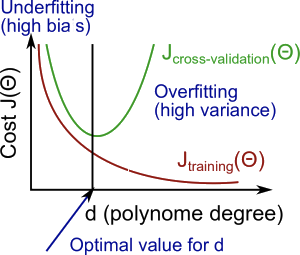
\includegraphics[scale=0.4]{./images/bias_and_variance_polynomial.png}
\end{center}

\noindent High bias(underfitting): both \(J_{train}(\Theta)\) and \(J_{cv}(\Theta)\) will be high. Also, \(J_{cv}(\Theta) \approx J_{train}(\Theta)\). 

\noindent High variance(overfitting): \(J_{train}(\Theta)\) will be low and \(J_{cv}(\Theta)\) will be high. Also, \(J_{cv}(\Theta) \gg J_{train}(\Theta)\). 

\bigskip

\noindent \textbf{Regularization:}

\noindent \(\lambda = 0\) causes overfitting. \(\lambda\) too large causes underfitting. To find a good \(\lambda\):

\begin{enumerate}
\item Create a list of lambdas (i.e. \(\lambda \in \{0, 0.1, 0.2, 0.4, 0.8, ..., 6.4 \}\)).
\item Create a set of models with different degrees or any other variants.
\item Iterate through the \(\lambda\)s and for each \(\lambda\) go through all the models to learn some \(\Theta\).
\item Compute the cross validation error using the learned \(\Theta\)(computed with \(\lambda\)) on the \(J_{cv}(\Theta)\).
\item Select the best combo that produces the lowest error on the cross validation set.
\item Using the best combo \(\Theta\) and \(\lambda\), apply it on \(J_{test}(\Theta)\) to see if it has a good generalization of the problem.
\end{enumerate}

\noindent \textbf{Learning curves:}

\noindent Training an algorithm on a very few number of data points (such as 1, 2 or 3) will easily have 0 errors because we can always find a quadratic curve that touches exactly those number of points. Hence:

\begin{itemize}
\item As the training set gets larger, the error for a quadratic function increases.
\item The error value will plateau out after a certain m, or training set size.
\end{itemize}

\noindent When Experiencing high bias:

\begin{center}
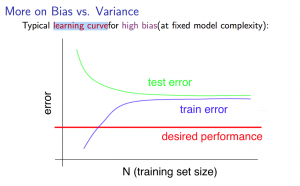
\includegraphics[scale=0.6]{./images/experiencing_high_bias.png}
\end{center}

\noindent Low training set size: \(J_{train}(\Theta)\) will be low and \(J_{cv}(\Theta)\) will be high.

\noindent Large training set size: both \(J_{train}(\Theta)\) and \(J_{cv}(\Theta)\) will be high, with \(J_{train}(\Theta) \approx J_{cv}(\Theta)\).

\noindent If a learning algorithm is suffering from high bias, getting more training data will not (by itself) help much.

\bigskip

\noindent When Experiencing high variance:

\begin{center}
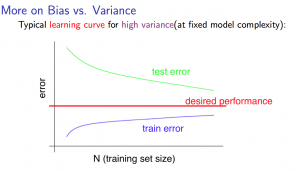
\includegraphics[scale=0.6]{./images/experiencing_high_variance.png}
\end{center}

\noindent Low training set size: \(J_{train}(\Theta)\) will be low and \(J_{cv}(\Theta)\) will be high.

\noindent Large training set size: \(J_{train}(\Theta)\) will increase and \(J_{cv}(\Theta)\) will decrease, with \(J_{train}(\Theta) < J_{cv}(\Theta)\) significantly.

\noindent If a learning algorithm is suffering from high variance, getting more training data is likely to help.

\bigskip

\noindent \textbf{Optimizing approaches:}

\begin{itemize}
\item Getting more training examples: Fixes high variance.
\item Trying smaller sets of features: Fixes high variance.
\item Adding features: Fixes high bias.
\item Adding polynomial features: Fixes high bias.
\item Decreasing \(\lambda\): Fixes high bias.
\item Increasing \(\lambda\): Fixes high variance.
\end{itemize}

\noindent \textbf{Diagnosing Neural Networks:}

\begin{itemize}
\item A neural network with fewer parameters is prone to underfitting. It is also computationally cheaper.
\item A large neural network with more parameters is prone to overfitting. It is also computationally expensive. In this case you can use regularization (increase \(\lambda\)) to address the overfitting.
\end{itemize}

\noindent Using a single hidden layer is a good starting default. You can train your neural network on a number of hidden layers using your cross validation set. You can then select the one that performs best.

\bigskip

\noindent \textbf{Model Complexity Effects:}

\begin{itemize}
\item Lower-order polynomials (low model complexity) have high bias and low variance. In this case, the model fits poorly consistently.
\item Higher-order polynomials (high model complexity) fit the training data extremely well and the test data extremely poorly. These have low bias on the training data, but very high variance.
\item In reality, we would want to choose a model somewhere in between, that can generalize well but also fits the data reasonably well.
\end{itemize}

\noindent \textbf{Recommended approach:}

\begin{itemize}
\item Start with a simple algorithm, implement it quickly, and test it early on your cross validation data.
\item Plot learning curves to decide if more data, more features, etc. are likely to help.
\item Manually examine the errors on examples in the cross validation set and try to spot a trend where most of the errors were made.
\end{itemize}

\noindent \textbf{Precision \& Recall: (deal with skewed classes)}

\noindent High \(F_{score} \in [0, 1]\) (high precision and high recall) represents a good prediction model.

\begin{center}
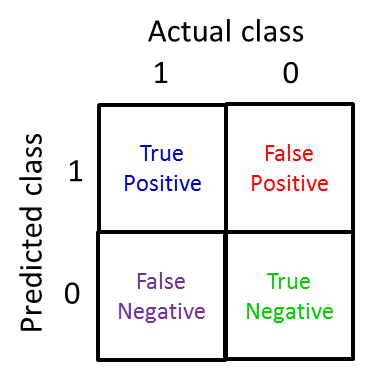
\includegraphics[scale=0.6]{./images/precision_recall.png}
\end{center}

\[\text{Precision} = \frac{\text{True positives}}{\text{predicted as positive}} = \frac{\text{True positives}}{\text{True positives + False positives}}\]
\[\text{Recall} = \frac{\text{True positives}}{\text{actual positives}} = \frac{\text{True positives}}{\text{True positives + False negatives}}\]
\[F_{score} = 2 \times \frac{\text{Precision} \times \text{Recall}}{\text{Precision + Recall}}\]

\section{Decision Tree}

\subsection{Classification}

\begin{center}
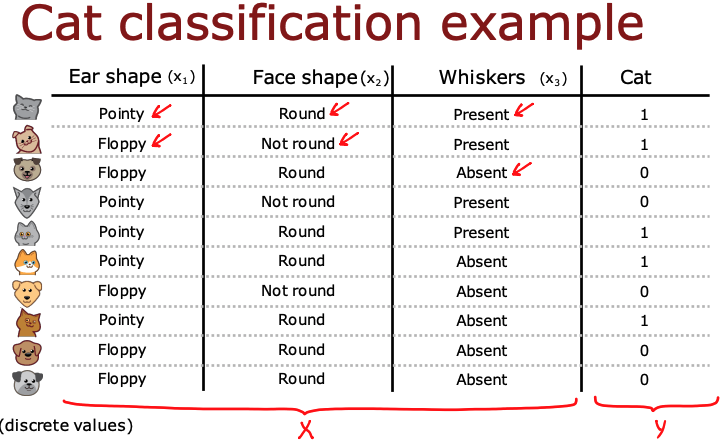
\includegraphics[scale=0.4]{./images/decision_tree_classification_data.png}
\end{center}

\begin{center}
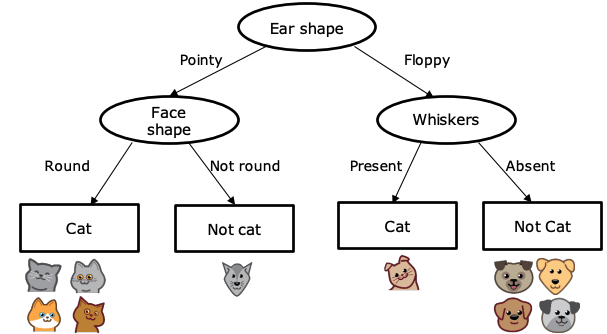
\includegraphics[scale=0.5]{./images/decision_tree_classification_process.png}
\end{center}

\noindent \textbf{root node}: The node on the top.

\bigskip

\noindent \textbf{decision node}: The node used to split data.

\bigskip

\noindent \textbf{leaf node}: The node on the bottom.

\bigskip

\noindent \textbf{node entropy}: Measure of the purity of the split data on nodes. Large if the data is not pure. Small if data is pure. Assume decision tree has \(K\) output classes. For \(i \in \{1, \dots, K\}\), \(p_k\) is the proportion of class \(k\) of all the data examples this node has.

\[{H}(node) = -\sum _{i=1}^{K}p_{k}\log _{2}p_{k}\]

\noindent \textbf{information gain}: Reduce of entropy from parent to children nodes. Assume parent node has \(C\) children, \(m_{p}\) data examples, entropy \({H}(p)\). Each child for \(c \in \{1, \dots, C\}\) has \(m_{c}\) data examples, entropy \({H}(c)\).

\[{IG}(parent, children) = H(p) - \sum _{c=1}^{C}\frac{m_{c}}{m_{p}}{H}(c)\]

\subsection{Regression}

\begin{center}
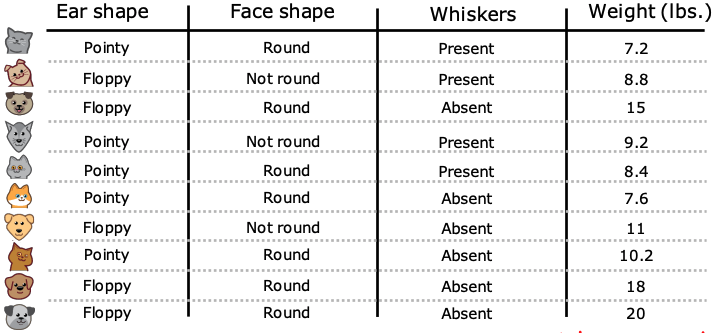
\includegraphics[scale=0.4]{./images/decision_tree_regression_data.png}
\end{center}

\begin{center}
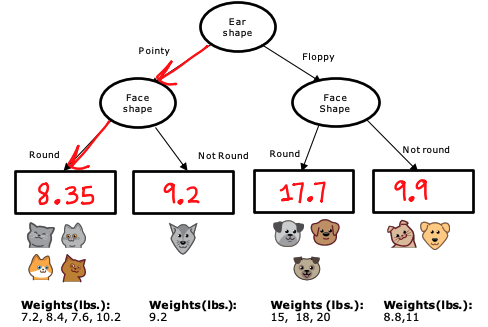
\includegraphics[scale=0.5]{./images/decision_tree_regression_process.png}
\end{center}

\noindent \textbf{node entropy.}: For regression problem, we can use variance of the outputs of the examples on node \(\sigma^{2}(node)\) as the entropy.

\[{H}(node) = \sigma^{2}(node)\]

\noindent \textbf{information gain}: Same expression as classification problem, just with different entropy.

\[{IG}(parent, children) = H(p) - \sum _{c=1}^{C}\frac{m_{c}}{m_{p}}{H}(c)\]

\subsection{Decision Tree Learning}

\noindent Notice that the decision tree splitting is a recursive process. Each of the children splits in the same way like their parents.

\begin{itemize}
    \item Start with all examples at the root node
    \item Calculate information gain for all possible features, and pick the one with
the highest information gain
    \item Split dataset according to selected feature, and create branches of the tree
    \item Keep repeating splitting process until stopping criteria is met:
    \begin{itemize}
        \item When a node is \(100\%\) one class
        \item When splitting a node will result in the tree exceeding a maximum
depth
        \item Information gain from additional splits is less than threshold
        \item When number of examples in a node is below a threshold
    \end{itemize}
\end{itemize}

\noindent \textbf{What if feature has multiple possible values?}

\noindent Use one-hot encoding to build training set. For example, if \textbf{Ear shape} has 3 possible values: \textbf{Pointy}, \textbf{Floppy}, \textbf{Oval}. We can add three features for each of the possible values to the training set, instead of adding \textbf{Ear shape} as a feature.

\bigskip

\noindent \textbf{What if feature is continuous?}

\noindent Use ranges of the feature to build training set. For example, \textbf{Weight} has a continuous value. We can add ranges: \(Weight \leq 0.8\), \(0.8 < Weight < 0.9\), \(Weight \geq 0.9\) as features to the training set.

\subsection{Decision Tree Prediction}

\noindent Feed an example to the root node. After the processing, the example will reach the leaf node.
\begin{itemize}
    \item \textbf{Classification}: The class \(k\) of the largest proportion \(p_{k}\) on leaf node on training examples is the prediction of decision tree.
    \item \textbf{Regression}: The average value of the outputs of training examples on the leaf node is the prediction of decision tree.
\end{itemize}

\subsection{Tree Ensembles}

Depending on the given training set, trained decision trees can be totally different and the performance can be unstable. Tree ensembles samples the training set randomly (sampling with replacement) to create multiple training sets with same size. With these training sets we can train multiple decision trees, and use them to do prediction. And take the final prediction based on the votes generated from different decision tree models.

\subsection{Random Forest Algorithm}

\noindent Given training set of size \(m\), for \(b \in \{1, \dots, B\}\) (\(B\) means "bags", the number of training sets we want to generate): use sampling with replacement to create a new training set of size \(m\),
then train a decision tree on the new dataset.

\bigskip

\noindent Randomizing the feature choice: at each node, when choosing a feature to use to split, if \(n\) features are available, pick a random subset of \(k < n\) features (can use \(k = \sqrt{n}\) when \(n\) is large) and allow the algorithm to only choose from that subset of features. This is to prevent the first a few level of tree using the same features at nodes even when the training set is randomly sampled. This helps to generate more different decision tree models.

\subsection{XGBoost (Extreme Gradient Boosting)}

\noindent Given training set of size \(m\), for \(b \in \{1, \dots, B\}\) (\(B\) means "bags", the number of training sets we want to generate): use sampling with replacement to create a new training set of size \(m\). \textbf{(But instead of picking from all examples with equal \(\frac{1}{m}\) probability, make it more likely to pick examples that the previously trained trees misclassify.)} Then train a decision tree on the new dataset. \textcolor{orange}{( * The sampling approach is complicated and not covered in this section.)}

\bigskip

\noindent This helps to make the training process focus on the training data that the decision tree currently cannot do well on.

\subsection{Decision Trees vs Neural Networks}

\noindent \textbf{Decision Trees and Tree ensembles}:
\begin{itemize}
    \item Works well on tabular (structured) data
    \item Not recommended for unstructured data (images, audio, text)
    \item Fast
    \item Small decision trees may be human interpretable
\end{itemize}

\noindent \textbf{Neural Networks}:
\begin{itemize}
    \item Works well on all types of data, including tabular (structured) and unstructured data
    \item May be slower than a decision tree
    \item Works with transfer learning
    \item When building a system of multiple models working together, it might be easier to string together multiple neural networks
\end{itemize}

\section{Unsupervised Learning}

\subsection{Clustering}

\noindent Clustering is the task of grouping a set of objects in such a way that objects in the same group (called a cluster) are more similar (in some sense) to each other than to those in other groups (clusters).

\subsubsection{K-means}

\begin{center}
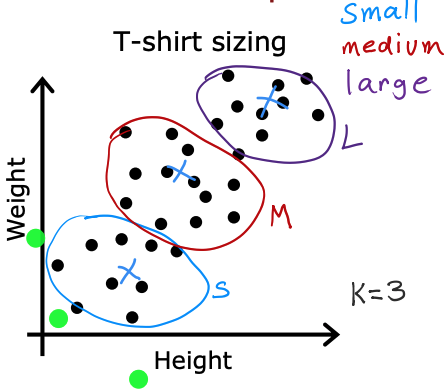
\includegraphics[scale=0.5]{./images/k_means_clustering.png}
\end{center}

\noindent \(K\): number of clusters we want to get.

\noindent \(c^{(i)}\): index of cluster \(\{1, \dots, K\}\) to which example \(x^{(i)}\) is currently assigned.

\noindent \(\mu_{k}\): cluster centroid of cluster \(k \in \{1, \dots, K\}\).

\noindent \(\mu_{c^{(i)}}\): cluster centroid of cluster to which example \(x^{(i)}\) has been assigned.

\noindent \textbf{cost function}:
\[J(c^{(1)}, \dots, c^{(m)}, \mu_{1}, \dots, \mu_{K}) = \frac{1}{m} \sum_{i = 1}^m  \vert\vert x^{(i)} - \mu_{c^{(i)}} \vert\vert^2\]

\noindent \textbf{Random initialization}: (reduce the chance of getting local optimum)

\noindent repeat 50 - 1000 times: \{

pick \(K\) random examples from the dataset as \(\{\mu_{1}, \dots, \mu_{K}\}\)

for \(i \in \{1, \dots, m\}\), \(c^{(i)} := \) index of cluster centroid closest to \(x^{(i)}\)

compute \(J(c^{(1)}, \dots, c^{(m)}, \mu_{1}, \dots, \mu_{K})\)

\noindent \}

\noindent then pick the set of clusters that gave lowest cost \(J\)

\bigskip

\noindent \textbf{Clustering process}:

\noindent repeat until convergence \{

\# assign points to cluster centroids

for \(i \in \{1, \dots, m\}\), \(c^{(i)} := \) index of cluster centroid closest to \(x^{(i)}\)

\# move cluster centroids

for \(k \in \{1, \dots, K\}\), \(\mu_{k} := \) average (mean) of points assigned to cluster \(k\)

\noindent \}

\bigskip

\noindent \textbf{How to choose \(K\)?}

\noindent We can use elbow method to pick the value of \(K\).

\begin{center}
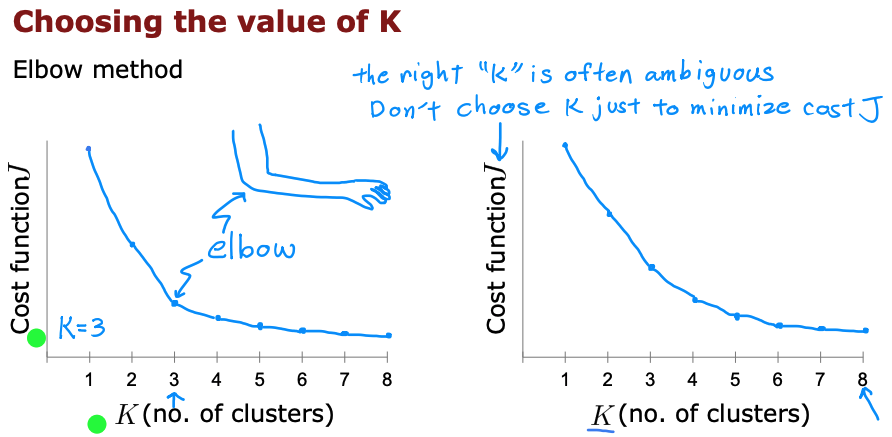
\includegraphics[scale=0.3]{./images/k_means_elbow_method.png}
\end{center}

\noindent Often, you want to get clusters for some later (downstream) purpose. Evaluate K-means based on how well it performs on that later purpose to choose the value of \(K\).

\begin{center}
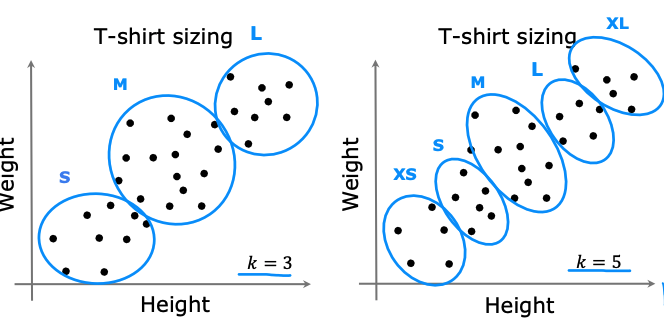
\includegraphics[scale=0.5]{./images/k_means_choose_k_later.png}
\end{center}

\subsection{Anomaly Detection}

\noindent Anomaly detection is generally understood to be the identification of rare items, events or observations which deviate significantly from the majority of the data and do not conform to a well defined notion of normal behaviour.

\bigskip

\noindent \textbf{Gaussian (Normal) Distribution}:

\[p(x) = \frac{1}{\sqrt{2\pi}\sigma} e^{\frac{-(x - \mu)^2}{2\sigma^2}}\]

\noindent \textbf{Anomaly Detection Algorithm}:

\begin{center}
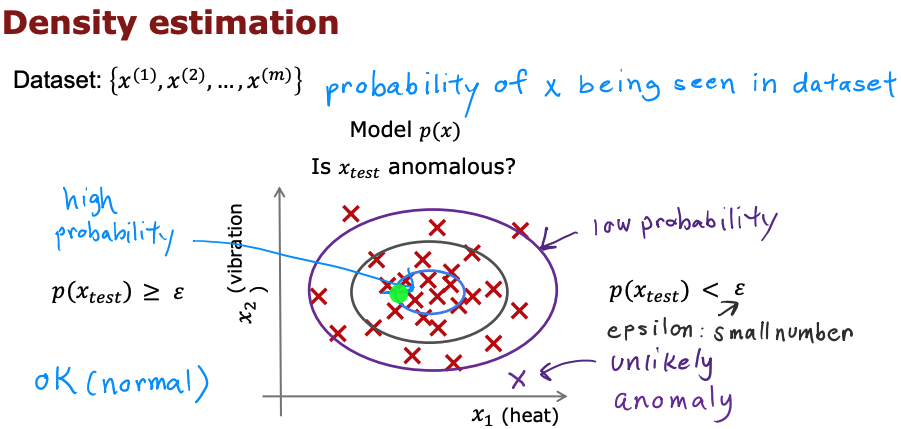
\includegraphics[scale=0.3]{./images/anomaly_detection_density_estimation.png}
\end{center}

\noindent Model normal distribution \(p(x)\) from data. Identify unusual data by checking which have \(p(x) < \epsilon\).

\[\mu = \frac{1}{m} \sum_{i = 1}^{m} x^{(i)}\]
\[\sigma^2 = \frac{1}{m} \sum_{i = 1}^{m} \vert\vert x^{(i)} - \mu \vert\vert^2\]
\[p(x) = \prod_{j = 1}^{n} p(x_{j}; \mu_{j}; \sigma_{j}^2) = \prod_{j = 1}^{n} \frac{1}{\sqrt{2\pi}\sigma_{j}} e^{\frac{-(x_{j} - \mu_{j})^2}{2\sigma_{j}^2}}\]
\[
y =
\begin{cases}
  1, & \text{if } p(x) < \epsilon \text{ (anomaly)} \\
  0, & \text{if } p(x) \geq \epsilon \text{ (normal)}
\end{cases}
\]

\bigskip

\noindent \textbf{training set}: \(m\) training examples with \(y = 0\) (non-anomalous).

\bigskip

\noindent \textbf{cross validation set}: \(m_{cv}\) examples with mostly \(y = 0\) (non-anomalous) and some \(y = 1\) (anomalous).

\bigskip

\noindent \textbf{test set}: \(m_{test}\) examples with mostly \(y = 0\) (non-anomalous) and some \(y = 1\) (anomalous).

\bigskip

\noindent \textbf{evaluation}: use \(F_1\) score for skewed dataset.

\bigskip

\noindent \textbf{Training Process}:

\noindent Fit model \(p(x)\) on training set. (get \(\mu, \sigma^2\))

\noindent On cross validation/test set, do evaluation and tune \(\epsilon, x_{j}\) to minimize \(F_1\) score. (choose the right threshold and features)

\bigskip

\noindent \textbf{Non-gaussian Features}:

\begin{center}
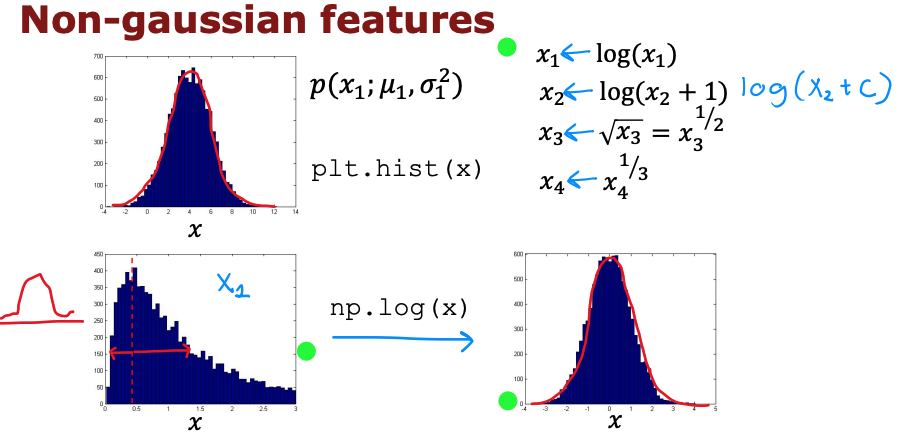
\includegraphics[scale=0.3]{./images/anomaly_detection_features.png}
\end{center}

\noindent We want the features fit gaussian distribution well. But features are not always normally distributed. We can process the features to make them normally distributed, for example: use \(log(x_{j} + c)\), \(x_{j}^{\frac{1}{c}}\) instead of \(x_{j}\).

\bigskip

\noindent The most common problem in anomaly detection is \(p(x)\) is similar for normal and anomalous examples. To solve this problem, we can choose features that might take on unusually large or small values in the event of an anomaly. These features can distinct anomalous examples from the normal ones.

\bigskip

\noindent Choose features based on \(p(x)\): large for normal examples, small for anomaly examples in the cross validation set.

\bigskip

\noindent For example: \(x_3\) is CPU load, \(x_4\) is network traffic. We can construct:

\[x_5 = \frac{(\text{CPU load})^2}{\text{network traffic}}\]

\bigskip

\noindent \textbf{Anomaly Detection vs. Supervised Learning}:

\noindent Use Anomaly detection if:

\begin{itemize}
    \item Very small number (0 to 20) of positive examples \(y = 1\); large number of negative examples \(y = 0\); Model \(p(x)\) with just negative examples. Use positive examples for cv and test sets.
    \item Many different “types” of anomalies. Hard for any algorithm to learn (from just positive examples) what the anomalies look like. Future anomalies may look nothing like any of the anomalous examples seen so far.
    \item e.g. Fraud detection; Manufacturing finding new previously unseen defects; Monitoring machines in a data center; Security applications.
\end{itemize}

\noindent Use Supervised Learning if:

\begin{itemize}
    \item Large number of positive and negative examples.
    \item Enough positive examples for algorithm to get a sense of what positive examples are like. Future positive examples likely to be similar to ones in training set.
    \item e.g. Email spam classification; Manufacturing finding known, previously seen defects; Weather prediction; Diseases classification.
\end{itemize}

\section{Recommender System}

\subsection{Collaborative Filtering}

\noindent collaborative filtering is a method of making automatic predictions (filtering) about the interests of a user by collecting preferences or taste information from many users (collaborating).

\begin{center}
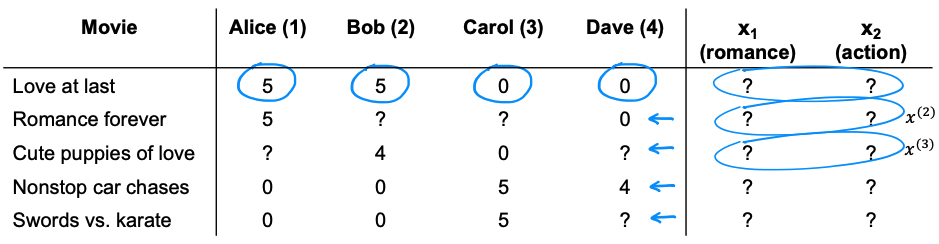
\includegraphics[scale=0.3]{./images/collaborative_filtering_data.png}
\end{center}

\noindent \(r(i, j)\): if user j has rated movie i (1 or 0)

\noindent \(y^{(i, j)}\): rating given by user j on movie i

\noindent \(w^{(j)}, b^{(j)}\): parameters for user j

\noindent \(x^{(i)}\): feature vector for movie i

\noindent \(m^{(j)}\): number of movies rated by user j

\noindent \(n_{m}\): number of movies

\noindent \(n_{u}\): number of users

\noindent \(n\): number of features

\bigskip

\noindent \textbf{predict rating}: (user j on movie i)

\[f_{(w, b, x)}(x^{(i)}) = w^{(j)} \cdot x^{(i)} + b^{(j)}\]

\noindent \textbf{cost function to learn}: \(\{w^{(1)}, b^{(1)}, \dots, w^{(n_u)}, b^{(n_u)}\}\)

\[J(w, b) = \frac{1}{2} \sum_{j = 1}^{n_u} \sum_{i:r(i, j)=1} (w^{(j)} \cdot x^{(i)} + b^{(j)} - y^{(i, j)})^2 + \frac{\lambda}{2} \sum_{j = 1}^{n_u} \sum_{k = 1}^{n} (w_{k}^{(j)})^2\]

\noindent \textbf{cost function to learn}: \(\{x^{(1)}, \dots, x^{(n_m)}\}\)

\[J(x) = \frac{1}{2} \sum_{i = 1}^{n_m} \sum_{j:r(i, j)=1} (w^{(j)} \cdot x^{(i)} + b^{(j)} - y^{(i, j)})^2 + \frac{\lambda}{2} \sum_{i = 1}^{n_m} \sum_{k = 1}^{n} (x_{k}^{(i)})^2\]

\noindent \textbf{cost function}: (combined)

\[J(w, b, x) = \frac{1}{2} \sum_{(i, j):r(i, j)=1} (w^{(j)} \cdot x^{(i)} + b^{(j)} - y^{(i, j)})^2 + \frac{\lambda}{2} \sum_{j = 1}^{n_u} \sum_{k = 1}^{n} (w_{k}^{(j)})^2 + \frac{\lambda}{2} \sum_{j = 1}^{n_m} \sum_{k = 1}^{n} (x_{k}^{(i)})^2\]

\noindent \textbf{Training Process}:

\noindent repeat until convergence \{
\[w_{i}^{(j)} = w_{i}^{(j)} - \alpha \frac{\partial}{\partial w_{i}^{(j)}} J(w, b, x)\]
\[b^{(j)} = b^{(j)} - \alpha \frac{\partial}{\partial b^{(j)}} J(w, b, x)\]
\[x_{k}^{(i)} = x_{k}^{(i)} - \alpha \frac{\partial}{\partial x_{k}^{(i)}} J(w, b, x)\]
\noindent \}

\bigskip

\noindent \textbf{Binary Labels}:

\noindent \textbf{predict like/unlike}: (user j on movie i)

\[f_{(w, b, x)}(x^{(i)}) = g(w^{(j)} \cdot x^{(i)} + b^{(j)})\]

\noindent \textbf{cost function}:

\[J(w, b, x) = \sum_{(i, j):r(i, j)=1} -y^{(i, j)} log(f_{(w, b, x)}(x^{(i)})) - (1 - y^{(i, j)})log(1 - f_{(w, b, x)}(x^{(i)}))\]

\noindent \textbf{Finding Related Items}:

\noindent Find item \(k\) with \(x^{(k)}\) similiar to \(x^{(i)}\) with smallest distance:

\[\vert\vert x^{(k)} - x^{(i)} \vert\vert^2 = \sum_{l=1}^{n} (x_{l}^{(k)} - x_{l}^{(i)})^2\]

\noindent \textbf{Limitations of Collaborative Filtering}:

\begin{itemize}
    \item Cold start problem
    \begin{itemize}
        \item How to rank new items that few users have rated?
        \item How to show something reasonable to new users who have rated few items?
    \end{itemize}
    \item Use side information about items or users
    \begin{itemize}
        \item Item: Genre, movie stars, studio, ...
        \item User: Demographics(age, gender, location), expressed
preferences, ...
    \end{itemize}
\end{itemize}

\subsection{Content-based Filtering}

\noindent Content-based filtering uses item features to recommend other items similar to what the user likes, based on their previous actions or explicit feedback.

\bigskip

\noindent We can construct 2 neural networks: user network, movie network. And then combine them, train them and make predictions.

\begin{center}
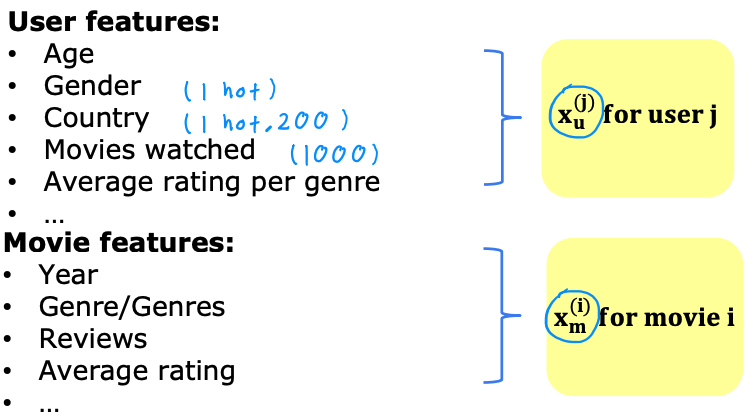
\includegraphics[scale=0.4]{./images/content_based_filtering_data.png}
\end{center}

\begin{center}
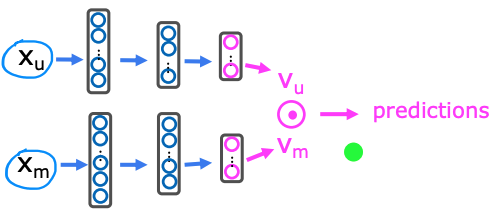
\includegraphics[scale=0.5]{./images/content_based_filtering_nn.png}
\end{center}

\noindent \(x_{u}\): user features.

\noindent \(x_{m}\): movie features.

\noindent \(v_{u}\): learned user vector.

\noindent \(v_{m}\): learned movie vector.

\bigskip

\noindent \textbf{cost function}:

\[J = \sum_{(i, j):r(i, j)=1} (v_{u}^{(j)} \cdot v_{m}^{(i)} - y^{(i, j)})^2 + \text{NN regularization term}\]

\noindent \textbf{Finding Related Items}:

\noindent To find movies similar to movie i with small distance:

\[\vert\vert v_{m}^{(k)} - v_{m}^{(i)} \vert\vert^2\]

\noindent \textbf{How to efficiently find recommendation from
a large set of items?}

\begin{itemize}
    \item Retrieval:
    \begin{itemize}
        \item Generate large list of plausible item candidates. For example:
        \begin{itemize}
            \item For each of the last 10 movies watched by the user, find 10 most similar movies
            \item For most viewed 3 genres, find the top 10 movies
            \item Top 20 movies in the country
        \end{itemize}
        \item Combine retrieved items into list, removing duplicates and items already watched/purchased
    \end{itemize}
    \item Ranking:
    \begin{itemize}
        \item Take list retrieved and rank using learned model 
        \item Display ranked items to user
    \end{itemize}
\end{itemize}

\noindent \textbf{Trade-off}:

\begin{itemize}
    \item Retrieving more items results in better performance, but slower recommendations.
    \item To analyse/optimize the trade-off, carry out offline experiments to see if retrieving additional items results in more relevant recommendations (i.e., \(p(y^{(i, j)}) = 1\) of items displayed to user are higher).
\end{itemize}

\subsection{Ethical Use of Recommender Systems}

\noindent The goal of the recommender system. Recommend:

\begin{itemize}
    \item Movies most likely to be rated 5 stars by user
    \item Products most likely to be purchased
    \item Ads most likely to be clicked on
    \item Products generating the largest profit
    \item Video leading to maximum watch time
\end{itemize}

\noindent However, sometimes we get recommender systems like:

\begin{itemize}
    \item Maximizing user engagement (e.g. watch time) has led to large social media/video sharing sites to amplify conspiracy theories and hate/toxicity
    \item Maximizing profit rather than users’ welfare
\end{itemize}

\noindent The ameliorations we can take:

\begin{itemize}
    \item Do not accept ads from exploitative businesses
    \item Filter out problematic content such as hate speech, fraud, scams and violent content
    \item Be transparent with users
\end{itemize}

\section{Reinforcement Learning}

\noindent Reinforcement learning (RL) is an area of machine learning concerned with how intelligent agents ought to take actions in an environment in order to maximize the notion of cumulative reward.

\subsection{Markov Chain}

\begin{center}
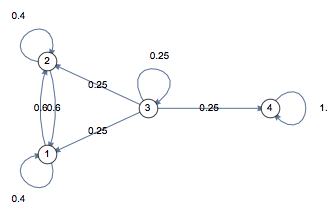
\includegraphics[scale=0.6]{./images/markov_chain_graph.png}
\end{center}

\noindent A Markov chain is a mathematical system that experiences transitions from one state to another according to certain probabilistic rules. The defining characteristic of a Markov chain is that no matter how the process arrived at its present state, the possible future states are fixed. In other words, the probability of transitioning to any particular state is dependent solely on the current state and time elapsed.

\subsection{Markov decision process}

\begin{center}
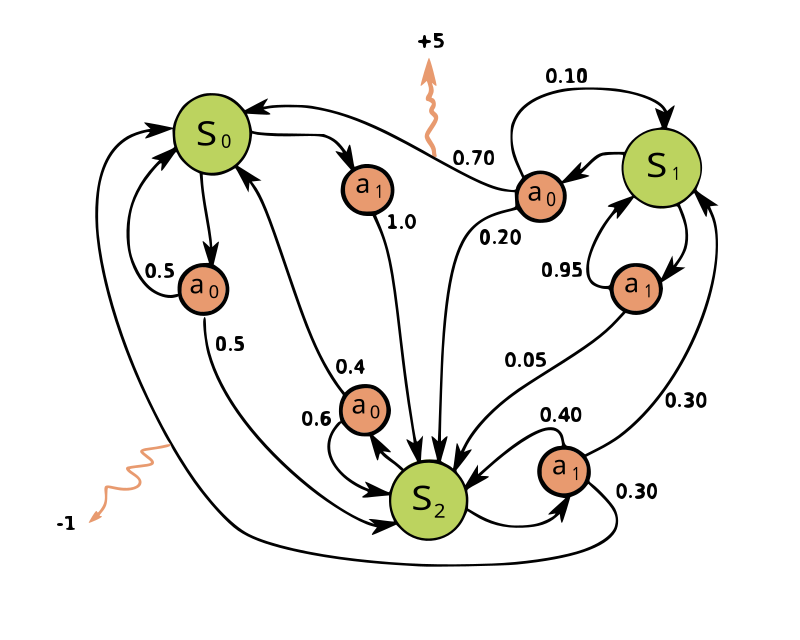
\includegraphics[scale=0.3]{./images/markov_decision_process.png}
\end{center}

\noindent A Markov decision process is a 4-tuple \((S,A,P_{a},R_{a})\), where:

\bigskip

\noindent \(S\): a set of states called the state space. The state space may be discrete or continuous, like the set of real numbers.

\noindent \(A\): a set of actions called the action space (alternatively, \(A_{s}\) is the set of actions available from state \(s\)). As for state, this set may be discrete or continuous.

\noindent \(P_{a}(s,s')\): on an intuitive level, the probability that action \(a\) in state \(s\) at time \(t\) will lead to state \(s'\) at time \(t+1\). In general, this probability transition is defined to satisfy: \(Pr(s_{t+1} \in S' \mid s_{t}=s, a_{t}=a) = \int_{S'} P_{a}(s,s') ds', S' \subseteq S\). In case the state space is discrete, the integral is intended with respect to the counting measure, so that the latter simplifies as \(P_{a}(s,s') = Pr(s_{t+1}=s' \mid s_{t}=s, a_{t}=a)\).

\noindent \(R_{a}(s,s')\): the immediate reward (or expected immediate reward) received after transitioning from state \(s\) to state \(s'\), due to action \(a\).

\bigskip

\noindent A policy function \(\pi\) is a (potentially probabilistic) mapping from state space \(S\) to action space \(A\).

\subsection{Q-learning}

\noindent For any finite Markov decision process (FMDP), Q-learning finds an optimal policy in the sense of maximizing the expected value of the total reward over any and all successive steps, starting from the current state. Q-learning can identify an optimal action-selection policy for any given FMDP, given infinite exploration time and a partly-random policy.

\bigskip

\noindent \(s\): current state.

\noindent \(a\): current action.

\noindent \(s'\): new state after taking action \(a\).

\noindent \(a'\): action chosen on state \(s'\).

\noindent \(\gamma\): discount factor.

\noindent \(\eta\): soft update factor.

\noindent \(episode\): a sequence of states, from an initial state to a terminal state.

\noindent \(experience\): agent's experience on a state \((s, a, R(s), s')\).

\noindent \(M\): number of episodes.

\noindent \(T\): maximum episode length (time steps) if episode doesn't terminate.

\noindent \(N\): memory buffer capacity to store experiences.

\noindent \(C\): number of time steps for update.

\noindent \(B\): batch size.

\noindent \(R(s)\): reward from state \(s\).

\noindent \(\epsilon\): greedy policy during training - with probability \(\epsilon\), pick an action randomly; with probability \(1 - \epsilon\), pick the action that maximizes \(Q(s, a)\). (can start high and reduce gradually during the training process)

\bigskip

\noindent \(Q(s, a)\): The expected cumulative reward for taking action \(a\) on state \(s\), then choosing actions for the following states that maximizes cumulative reward.

\[Q(s, a) = R(s) + \gamma \max_{a'} Q(s', a')\]

\noindent \(\pi(s)\): a policy that given state \(s\), returns best action that maximizes the cumulative reward from state \(s\) onward.

\[\pi(s) = \underset{a}{argmax} \ Q(s, a)\]

\noindent \textbf{Training data}: get \((s_{i}, a_{i}, R(s_{i}), s_{i+1})\) experience tuple from environment.

\[x^{(i)} = s_{i}\]
\[
y^{(i)} =
\begin{cases}
  R(s_{i}), & \text{for terminal } s_{i+1} \\
  R(s_{i}) + \gamma \ \underset{a_{i+1}}{max} \ Q(s_{i+1}, a_{i+1}), & \text{for non-terminal } s_{i+1}
\end{cases}
\]

\noindent \textbf{Cost function}:

\[J(w, b) = \frac{1}{2m} \sum_{i = 1}^m (Q(s_{i}, a_{i}) - y^{(i)})^2\]

\noindent \textbf{Random (stochastic) environment?}

\noindent In a stochastic environment, after taking an action, the next state can have multiple possibilities. For example, after taking action \(a\), there is 0.1 chance that we get state \(s_1\), 0.2 chance to get state \(s_2\), and 0.7 chance to get state \(s_3\). To solve this problem, we can take the expectation of following cumulative reward:

\[Q(s, a) = R(s) + \gamma E[\max_{a'} Q(s', a')]\]

\noindent \textbf{Learning Process}:

\begin{center}
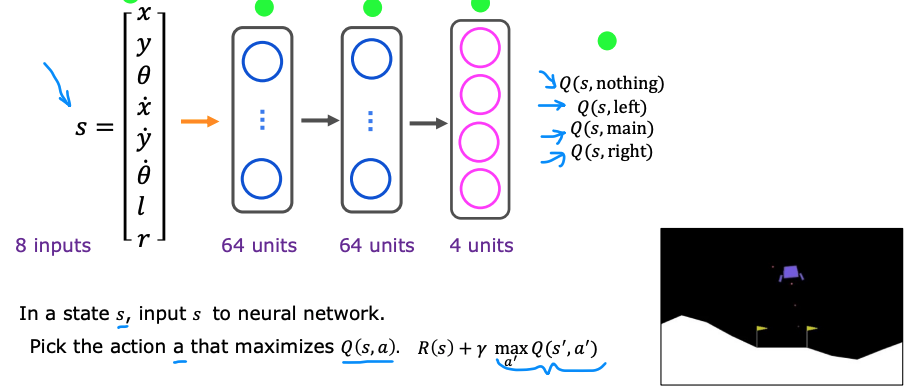
\includegraphics[scale=0.3]{./images/q_learning_nn.png}
\end{center}

\noindent Initialize memory buffer with capacity \(N\).

\noindent Initialize Q-network with random \(w, b\) as a guess of \(Q(s, a)\).

\noindent for \(i \in \{1, \dots, M\}\):

\noindent \hspace{.5cm} Receive initial state \(s_1\).

\noindent \hspace{.5cm} for \(t \in \{1, \dots, T\}\):

\noindent \hspace{1cm} Choose \(a_{t}\) for \(s_{t}\) with greedy policy \(\epsilon\).

\noindent \hspace{1cm} Get \((s_{t}, a_{t}, R(s_{t}), s_{t+1})\) experience tuple from environment.

\noindent \hspace{1cm} Store experience tuple in memory buffer, first in first out.

\bigskip

\noindent \hspace{1cm} Every \(C\) time steps perform a learning update:

\noindent \hspace{1cm} Sample \(B\) random experiences from memory buffer.

\noindent \hspace{1cm} For \((s_{j}, a_{j}, R(s_{j}), s_{j+1})\), \(j \in \{1, \dots, B\}\), construct training sample:

\[x^{(j)} = s_{j}\]
\[
y^{(j)} =
\begin{cases}
  R(s_{j}), & \text{for terminal } s_{j+1} \\
  R(s_{j}) + \gamma \ \underset{a_{j+1}}{max} \ Q(s_{j+1}, a_{j+1}), & \text{for non-terminal } s_{j+1}
\end{cases}
\]

\noindent \hspace{1cm} Train \(Q_{new}\) such that \(Q_{new}(s, a) \approx y\):

\noindent \hspace{1cm} Perform a gradient descent with mini batch and implement soft update:

\[w = (1 - \eta)w + \eta w_{new}\]
\[b = (1 - \eta)b + \eta b_{new}\]

\bigskip

\noindent \hspace{1cm} Start a new episode if \(s_{t+1}\) terminates, else continue.

\subsection{Policy Gradient}

\noindent \textbf{On-policy vs Off-policy learning}:

\noindent The key difference lies in how these methods approach learning:

\begin{itemize}
    \item On-policy:
    \begin{itemize}
        \item Training data is only generated from the exact same policy. e.g. Policy Gradient
        \item Learn from your own current strategy (even if it's not the best one yet).
    \end{itemize}
    \item Off-policy:
    \begin{itemize}
        \item Training data can originate from other sources that are not from the exact same policy. e.g. Q-learning, with greedy policy \(\epsilon\) in training, without \(\epsilon\) in prediction
        \item Learn from a different strategy (potentially better or more informed) than what you're currently using.
    \end{itemize}
    \item The primary distinction lies in how they approach exploration and exploitation, which affects their convergence properties and practical performance in different types of environments.
\end{itemize}

\noindent \textbf{Policy Gradient Algorithms}:

\noindent TBD: https://lilianweng.github.io/posts/2018-04-08-policy-gradient/

\subsection{Monte Carlo tree search (MCTS)}

\noindent The focus of MCTS is on the analysis of the most promising moves, expanding the search tree based on random sampling of the search space. The application of Monte Carlo tree search in games is based on many playouts, also called roll-outs. In each playout, the game is played out to the very end by selecting moves at random. The final game result of each playout is then used to weight the nodes in the game tree so that better nodes are more likely to be chosen in future playouts.

\bigskip

\noindent The most basic way to use playouts is to apply the same number of playouts after each legal move of the current player, then choose the move which led to the most victories. The efficiency of this method—called Pure Monte Carlo Game Search—often increases with time as more playouts are assigned to the moves that have frequently resulted in the current player's victory according to previous playouts. Each round of Monte Carlo tree search consists of four steps:

\begin{itemize}
    \item Selection: Start from root \(R\) and select successive child nodes until a leaf node \(L\) is reached. The root is the current game state and a leaf is any node that has a potential child from which no simulation (playout) has yet been initiated. \(L = R\) at the beginning of the search. The section below says more about a way (UCT) of biasing choice of child nodes that lets the game tree expand towards the most promising moves, which is the essence of Monte Carlo tree search.
    \item Expansion: Unless \(L\) ends the game decisively (e.g. win/loss/draw) for either player, create one (or more) child nodes. Child nodes are any valid moves from the game position defined by \(L\).
    \item Simulation: For each node \(C\) from the expanded nodes, complete one random playout from node \(C\). This step is sometimes also called playout or rollout. A playout may be as simple as choosing uniform random moves until the game is decided (for example in chess, the game is won, lost, or drawn).
    \item Backpropagation: Use the result of the playout to update information in the nodes on the path from \(C\) to \(R\).
\end{itemize}

\begin{center}
    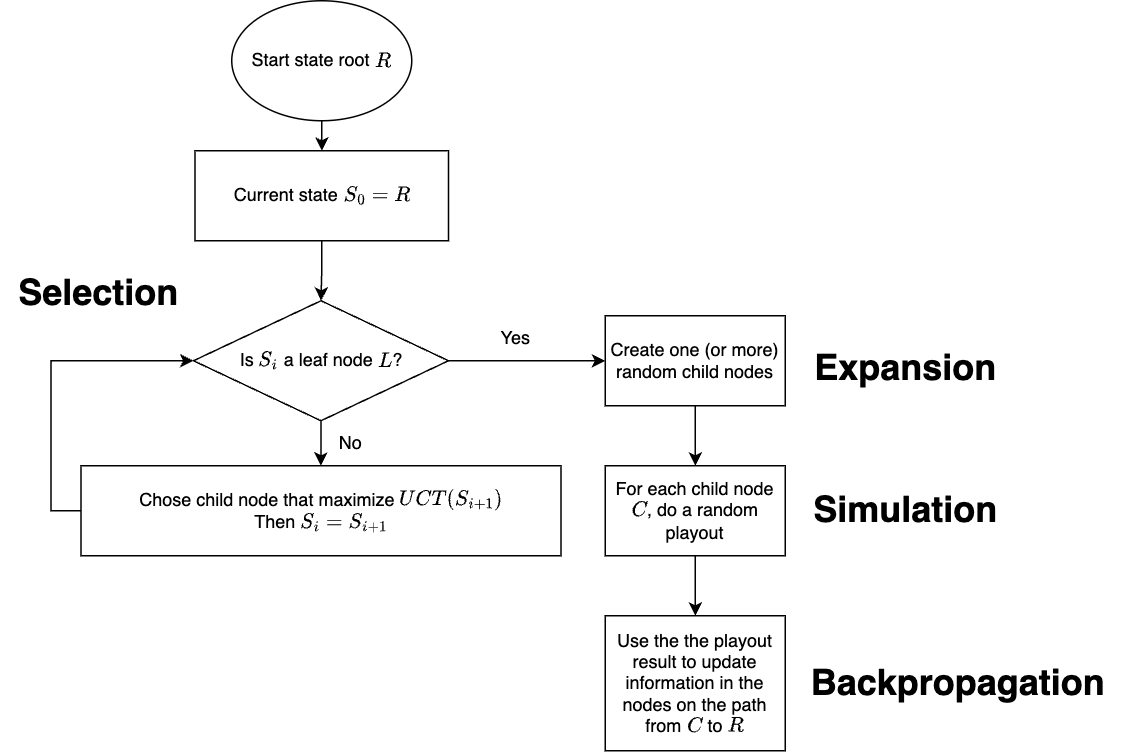
\includegraphics[scale=0.2]{./images/mcts_flow.png}
\end{center}

\begin{center}
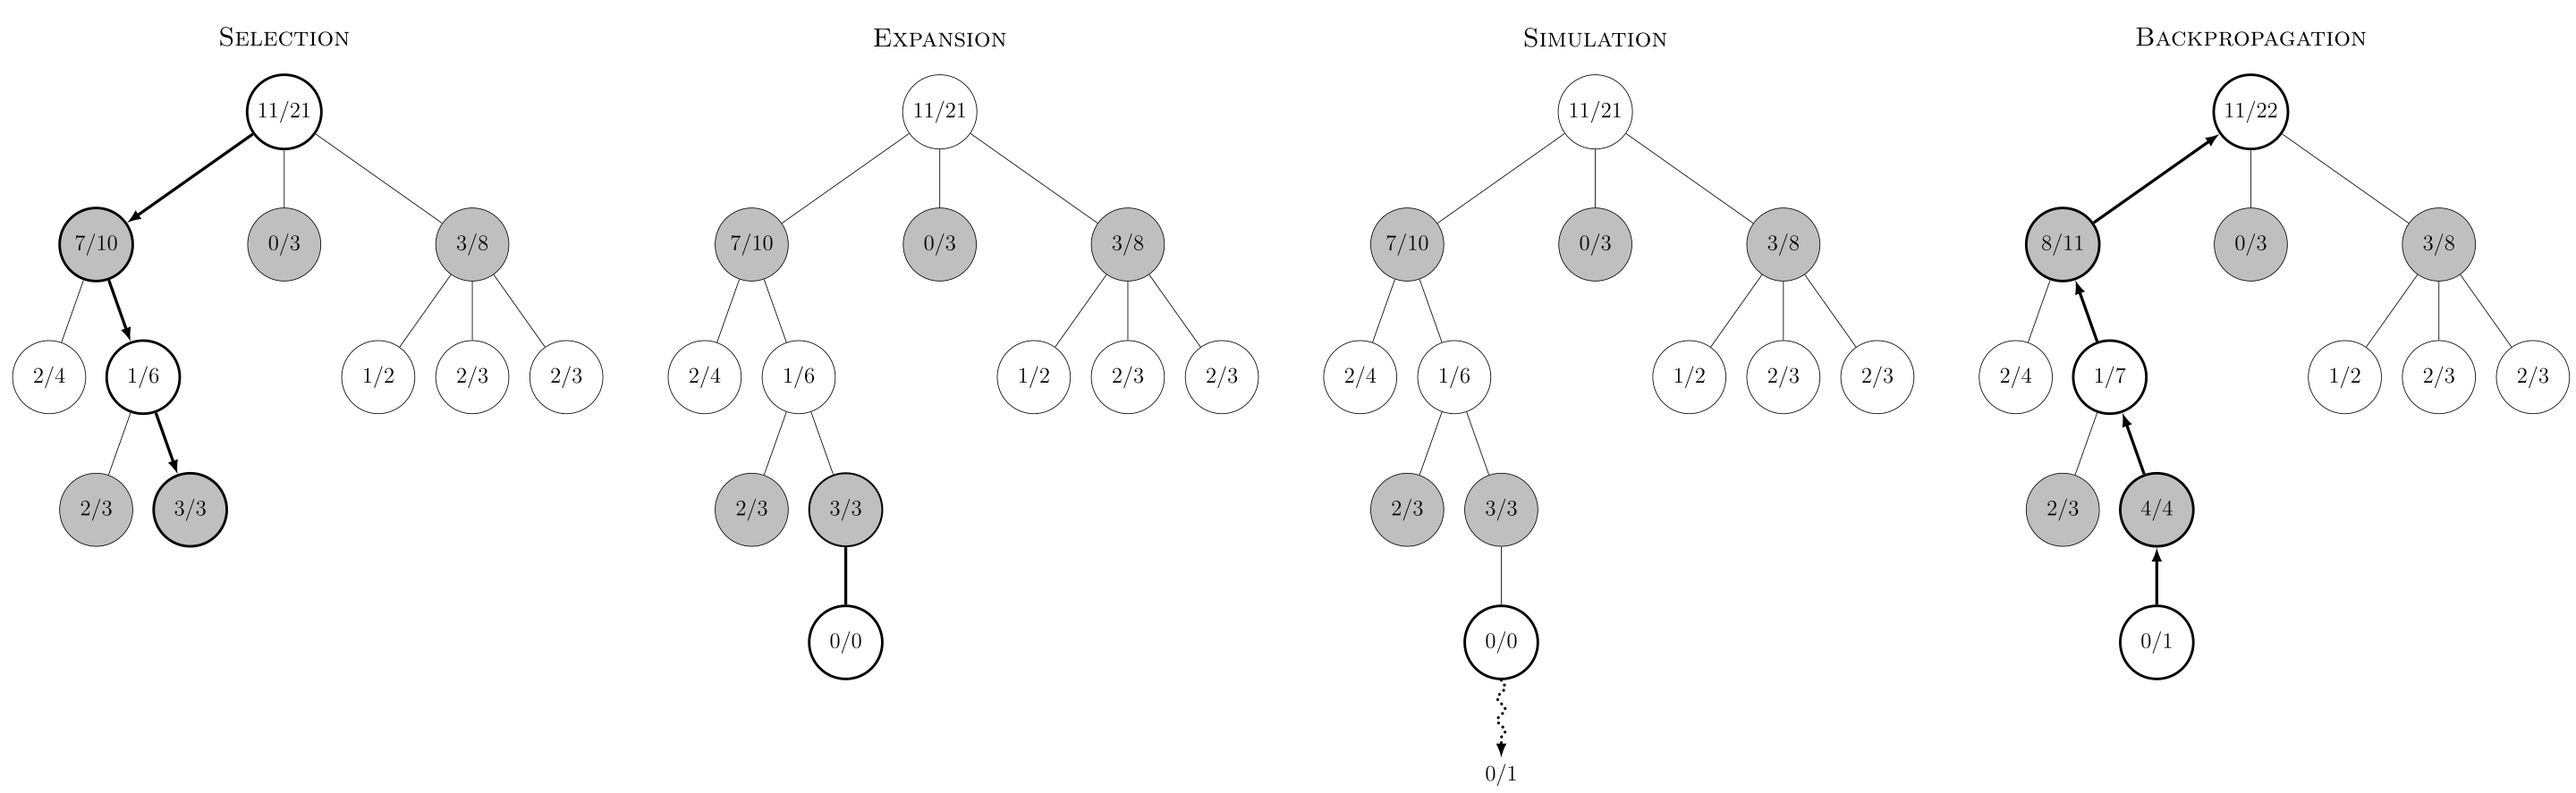
\includegraphics[scale=0.1]{./images/mcts_steps.png}
\end{center}

\noindent This graph shows the steps involved in one decision, with each node showing the ratio of wins to total playouts from that point in the game tree for the player that the node represents. In the Selection diagram, black is about to move. The root node shows there are 11 wins out of 21 playouts for white from this position so far. It complements the total of 10/21 black wins shown along the three black nodes under it, each of which represents a possible black move. Note that this graph does not follow the UCT algorithm described below.

\bigskip

\noindent If white loses the simulation, all nodes along the selection incremented their simulation count (the denominator), but among them only the black nodes were credited with wins (the numerator). If instead white wins, all nodes along the selection would still increment their simulation count, but among them only the white nodes would be credited with wins. In games where draws are possible, a draw causes the numerator for both black and white to be incremented by 0.5 and the denominator by 1. This ensures that during selection, each player's choices expand towards the most promising moves for that player, which mirrors the goal of each player to maximize the value of their move.

\bigskip

\noindent Rounds of search are repeated as long as the time allotted to a move remains. Then the move with the most simulations made (i.e. the highest denominator) is chosen as the final answer.

\bigskip

\noindent DeepMind's AlphaZero replaces the simulation step with an evaluation based on a neural network.

\bigskip

\noindent \textbf{UCT (Upper Confidence Bound 1 applied to trees):}

\bigskip

\noindent The main difficulty in selecting child nodes is maintaining some balance between the exploitation of deep variants after moves with high average win rate and the exploration of moves with few simulations. The first formula for balancing exploitation and exploration in games is called UCT. UCT recommends to choose in each node of the game tree the move for which the following expression has the highest value:

\[\frac{w_{i}}{n_{i}} + c \sqrt{\frac{ln N_{i}}{n_i}}\]

\begin{itemize}
    \item \(w_{i}\) stands for the number of wins for the node considered after the i-th move
    \item \(n_{i}\) stands for the number of simulations for the node considered after the i-th move
    \item \(N_{i}\) stands for the total number of simulations after the i-th move run by the parent node of the one considered
    \item \(c\) is the exploration parameter—theoretically equal to \(\sqrt{2}\); in practice usually chosen empirically
\end{itemize}

\noindent The first component of the formula above corresponds to exploitation; it is high for moves with high average win ratio. The second component corresponds to exploration; it is high for moves with few simulations.

\printindex

\end{document}